\documentclass{beamer}
\usetheme[white]{Wisconsin}
\usepackage{longtable}
\usepackage{listings}
\usepackage{color}
%% The amssymb package provides various useful mathematical symbols
\usepackage{amssymb}
%% The amsthm package provides extended theorem environments
\usepackage{amsthm} \usepackage{amsmath} \usepackage{tmadd,tmath}
\usepackage[mathcal]{euscript} \usepackage{color}
\usepackage{textcomp}
\usepackage{algorithm,algorithmic}
\definecolor{listinggray}{gray}{0.9}
\definecolor{lbcolor}{rgb}{0.9,0.9,0.9}
\lstset{
  backgroundcolor=\color{lbcolor},
  tabsize=4,
  rulecolor=,
  language=c++,
  basicstyle=\scriptsize,
  upquote=true,
  aboveskip={1.5\baselineskip},
  columns=fixed,
  showstringspaces=false,
  extendedchars=true,
  breaklines=true,
  prebreak =
  \raisebox{0ex}[0ex][0ex]{\ensuremath{\hookleftarrow}},
  frame=single,
  showtabs=false,
  showspaces=false,
  showstringspaces=false,
  identifierstyle=\ttfamily,
  keywordstyle=\color[rgb]{0,0,1},
  commentstyle=\color[rgb]{0.133,0.545,0.133},
  stringstyle=\color[rgb]{0.627,0.126,0.941},
}

%% colors
\setbeamercolor{boxheadcolor}{fg=white,bg=UWRed}
\setbeamercolor{boxbodycolor}{fg=black,bg=white}


%%---------------------------------------------------------------------------%%
\author{Stuart R. Slattery
  \\ Engineering Physics Department
  \\ University of Wisconsin - Madison
}

\date{\today} 
\title{Massively Parallel Monte Carlo Methods for Discrete Linear and
  Nonlinear Systems} 
\begin{document}
\maketitle

%%---------------------------------------------------------------------------%%
\begin{frame}{Introduction}

  \begin{itemize}
  \item Predictive modeling and simulation enhances engineering
    capability
  \item Modern work focused on this task leverages multiple physics
    simulation (CASL, NEAMS)
  \item New hardware drives algorithm development (petascale and
    exascale)
  \item Monte Carlo methods have the potential to provide great
    improvements that permit finer simulations and better mapping to
    future hardware
  \item A set of massively parallel Monte Carlo methods is proposed to
    advance multiple physics simulation on contemporary and future
    leadership class machines
  \end{itemize}

\end{frame}

%%---------------------------------------------------------------------------%%
\begin{frame}{Physics-Based Motivation}
  
  \begin{beamerboxesrounded}[upper=boxheadcolor,lower=boxbodycolor,shadow=true]
    {Predictive nuclear reactor analysis enables...}
    \begin{itemize}
    \item Tighter design tolerance for improved thermal performance
      and efficiency
    \item Higher fuel burn-up
    \item High confidence in accident scenario models
    \end{itemize}
  \end{beamerboxesrounded}

  \begin{beamerboxesrounded}[upper=boxheadcolor,lower=boxbodycolor,shadow=true]
    {Multiple physics simulations are complicated...}
    \begin{itemize}
    \item Neutronics, thermal hydraulics, computational fluid
      dynamics, structural mechanics, and many other physics
    \item Consistent models yield nonlinearities in the variables
      through feedback effects
    \item Tremendous computational resources are required with
      $O(\sn{1}{9})$ element meshes and $O(100,000)+$ cores used in
      today's simulations.
    \end{itemize}
  \end{beamerboxesrounded}

\end{frame}

%%---------------------------------------------------------------------------%%
\begin{frame}{Physics-Based Motivation: DNB}

  \begin{columns}

    \begin{column}{0.35\textwidth}
      \begin{figure}[htpb!]
        \begin{center}
          \scalebox{1}{ \input{dnb_schematic.pdftex_t} }
        \end{center}
        \caption{\textbf{Departure from nucleate boiling scenario.} }
      \end{figure}
    \end{column}

    \begin{column}{0.65\textwidth}
      \begin{figure}[htpb!]
        \begin{center}
          \scalebox{0.8}{ \input{dnb_example.pdftex_t} }
        \end{center}
        \caption{\textbf{Multiphysics dependency analysis of departure
            from nucleate boiling.} }
      \end{figure}
    \end{column}

  \end{columns}

\end{frame}

%%---------------------------------------------------------------------------%%
\begin{frame}{Hardware-Based Motivation}

  \begin{itemize}
  \item Modern hardware is moving in two directions:
    \begin{itemize}
    \item Lightweight machines
    \item Heterogeneous machines
    \item Both characterized by low power and high concurrency
    \end{itemize}
  \item Some issues:
    \begin{itemize}
    \item Higher potential for both soft and hard failures
    \item Memory restrictions are expected with a continued decrease
      in memory/FLOPS
    \end{itemize}
  \item Potential resolution from Monte Carlo:
    \begin{itemize}
    \item Soft failures buried within the tally variance
    \item Hard failures are high variance events
    \item Memory savings over conventional methods
    \end{itemize}
  \end{itemize}

\end{frame}

%%---------------------------------------------------------------------------%%
\begin{frame}{Research Outline}
  \begin{itemize}
  \item Parallelization of Monte Carlo methods for discrete systems
    \begin{itemize}
    \item Parallel strategies taken from modern reactor physics
      methods
    \item Research is required to explore varying parallel strategies
    \item Scalability is of concern
    \end{itemize}
  \item Development of a nonlinear solver for discrete systems
    leveraging Monte Carlo
    \begin{itemize}
    \item Application to nonlinear problems of interest
    \item Memory benefits
    \item Performance benefits
    \end{itemize}
  \end{itemize}
\end{frame}

%%---------------------------------------------------------------------------%%
\begin{frame}{Linear Operator Equations}

  \begin{itemize}
  \item We seek solutions of the general linear operator equation
  \end{itemize}

  \[
  \ve{A} \ve{x} = \ve{b}
  \]
  \[
  \ve{A} \in \mathbb{R}^{N \times N},\ \ve{A} : \mathbb{R}^{N}
  \rightarrow \mathbb{R}^{N},\ \ve{x} \in \mathbb{R}^N,\ \ve{b} \in
  \mathbb{R}^N
  \]


  \[
  \ve{r} = \ve{b} - \ve{A}\ve{x}
  \]

  \begin{itemize}
  \item $\ve{r}=\ve{0}$ when an exact solution is found
  \end{itemize}

  \begin{beamerboxesrounded}[upper=boxheadcolor,lower=boxbodycolor,shadow=true]
    {A Requirement} Assert that $\ve{A}$ is \textit{nonsingular}. The
    solution is then:
    \[
    \ve{x} = \ve{A}^{-1}\ve{b}
    \]
  \end{beamerboxesrounded}

\end{frame}

%%---------------------------------------------------------------------------%%
\begin{frame}{Projection Methods}

  \begin{itemize}
  \item Powerful class of iterative methods (Saad,2003)
  \item Provides theory that encapsulates most other iterative methods
  \item Leveraged in many modern physics codes at the petascale
  \end{itemize}

  \begin{beamerboxesrounded}[upper=boxheadcolor,lower=boxbodycolor,shadow=true]
    {Search Subspace $\mathcal{K}$} Extract the solution from the
    search subspace:
    \[
    \tilde{\ve{x}} = \ve{x}_0 +
    \boldsymbol{\delta},\ \boldsymbol{\delta} \in \mathcal{K}
    \]
  \end{beamerboxesrounded}

  \begin{beamerboxesrounded}[upper=boxheadcolor,lower=boxbodycolor,shadow=true]
    {Constraint Subspace $\mathcal{L}$} Constrain the extraction with
    the constraint subspace by asserting orthogonality with the
    residual:
    \[
    \langle \tilde{\ve{r}},\ve{w} \rangle = 0,\ \forall \ve{w} \in
    \mathcal{L}
    \]  
  \end{beamerboxesrounded}

\end{frame}

%%---------------------------------------------------------------------------%%
\begin{frame}{The Orthogonality Constraint}

  \[
  \tilde{\ve{r}} = \ve{r}_0 - \ve{A}\boldsymbol{\delta}
  \]

  \begin{figure}[htpb!]
    \begin{center}
      \scalebox{1.1}{ \input{orthogonal_residual.pdftex_t} }
    \end{center}
    \caption{\textbf{Orthogonality constraint of the new residual with
        respect to $\mathcal{L}$.}}
  \end{figure}

  \begin{beamerboxesrounded}[upper=boxheadcolor,lower=boxbodycolor,shadow=true]
    {Minimization Property}

    The residual of the system is \textit{minimized} with respect to
    the constraints
    \[
    ||\tilde{\ve{r}}||_2 \leq ||\ve{r}_0||_2,\ \forall \ve{r}_0 \in
    \mathbb{R}^N
    \]
  \end{beamerboxesrounded}

\end{frame}

%%---------------------------------------------------------------------------%%
\begin{frame}{Krylov Subspace Methods}

  \[
  \mathcal{K}_m(\ve{A},\ve{r}_0) = span\{\ve{r}_0, \ve{A}\ve{r}_0,
  \ve{A}^2\ve{r}_0, \dots, \ve{A}^{m-1}\ve{r}_0\}
  \]

  \begin{itemize}
  \item For GMRES (Saad, 1986):
  \end{itemize}
  \[
  \mathcal{L} = \ve{A} \mathcal{K}_m(\ve{A},\ve{r}_0)
  \]

  \begin{itemize}
  \item Yields the normal system $\ve{A}^T\ve{A}\ve{x} =
    \ve{A}^T\ve{b}$
  \item Must generate an orthonormal basis for
    $\mathcal{K}_m(\ve{A},\ve{r}_0)$
  \item Typically choose a Gram-Schmidt-like procedure such as Arnoldi
    or Lanzcos
  \item Short and long recurrence relations available for
    orthogonalization
  \end{itemize}

\end{frame}

%%---------------------------------------------------------------------------%%
\begin{frame}{Parallel Projection Methods}
  
  \begin{itemize}
  \item Parallel vector update
  \end{itemize}
  \[
  \ve{y}[n] \leftarrow \ve{y}[n] + a * \ve{x}[n],\ \forall n \in
     [1,N_g]
  \]
  \[
  \ve{y}[n] \leftarrow \ve{y}[n] + a * \ve{x}[n],\ \forall n \in
     [1,N_l]
  \]
  
  \begin{itemize}
  \item Parallel dot product
  \end{itemize}
  \[
  d_l = \ve{y}_l \cdot \ve{x}_l,\ d_g = \sum_p d_l
  \]

  \begin{itemize}
  \item Parallel vector norm
  \end{itemize}
  \[
  ||x||_{\infty,l} = \max_n \ve{y}[n],\ \forall n \in [1,N_l]
  \]
  \[
  ||x||_{\infty,g} = \max_p ||x||_{\infty,l}
  \]
  
\end{frame}

%%---------------------------------------------------------------------------%%
\begin{frame}{Parallel Matrix-Vector Multiplication}

  \begin{figure}[htpb!]
    \begin{center}
      \scalebox{0.6}{ \input{partitioned_matrix.pdftex_t} }
    \end{center}
    \caption{\textbf{Matrix-vector multiply $\ve{A}\ve{x}=\ve{y}$
        operation on 3 processors.}
      \label{fig:partitioned_matvec_multiply} }
  \end{figure}

  \begin{figure}[htpb!]
    \begin{center}
      \scalebox{0.7}{ \input{matvec_proc_1.pdftex_t} }
    \end{center}
    \caption{\textbf{Components of multiply operation owned by process
        1.} }
    \label{fig:matvec_proc_1}
  \end{figure}

\end{frame}

%%---------------------------------------------------------------------------%%
\begin{frame}{Projection Methods Summary}

  \begin{itemize}
  \item Widely used in practice
  \item Krylov methods require only the action of the operator
  \item Parallelism achieved through a handful of operations
  \item Global reduction operations observed not to impede scalability
    (Gropp,2001)
    \begin{itemize}
    \item Dot product
    \item Vector norms
    \end{itemize}
  \item Nearest neighbor computations have poor algorithmic strong
    scaling
    \begin{itemize}
    \item Matrix-vector multiply
    \item Weak scaling is better
    \end{itemize}
  \item Short and long recurrence relations available for
    orthogonalization
  \end{itemize}

\end{frame}

%%---------------------------------------------------------------------------%%
\begin{frame}{Monte Carlo Methods for Discrete Linear Systems}

  \begin{itemize}
  \item First proposed by J. Von Neumann and S.M. Ulam in the 1940's
  \item Earliest published reference in 1950
  \item General lack of published work
  \item Modern work by Evans and others has yielded new applications
  \end{itemize}
\end{frame}

%%---------------------------------------------------------------------------%%
\begin{frame}{Monte Carlo Linear Solver Preliminaries}

  \begin{itemize}
  \item Split the operator
  \end{itemize}

  \[
  \ve{H} = \ve{I} - \ve{A}
  \]

  \[
  \ve{x} = \ve{H} \ve{x} + \ve{b}
  \]

  \begin{itemize}
  \item Generate the \textit{Neumann series}
  \end{itemize}
  
  \[
  \ve{A}^{-1} = (\ve{I}-\ve{H})^{-1} = \sum_{k=0}^{\infty} \ve{H}^k
  \]

  \begin{itemize}
  \item Require $\rho(\ve{H}) < 1$ for convergence
  \end{itemize}

  \[
  \ve{A}^{-1}\ve{b} = \sum_{k=0}^{\infty} \ve{H}^k\ve{b} = \ve{x}
  \]

\end{frame}

%%---------------------------------------------------------------------------%%
\begin{frame}{Monte Carlo Linear Solver Preliminaries}

  \begin{itemize}
  \item Expand the Neumann series
  \end{itemize}

  \[
  x_i = \sum_{k=0}^{\infty}\sum_{i_1}^{N}\sum_{i_2}^{N}\ldots
  \sum_{i_k}^{N}h_{i,i_1}h_{i_1,i_2}\ldots h_{i_{k-1},i_k}b_{i_k}
  \]

  \begin{itemize}
  \item Define a sequence of state transitions
  \end{itemize}
  
  \[
  \nu = i \rightarrow i_1 \rightarrow \cdots \rightarrow i_{k-1}
  \rightarrow i_{k}
  \]

  \begin{itemize}
  \item Define the \textit{Neumann-Ulam decomposition}\footnote{The
    Hadamard product $\ve{A} = \ve{B} \circ \ve{C}$ is defined
    element-wise as $a_{ij} = b_{ij} c_{ij}$.}
  \end{itemize}

  \[
  \ve{H} = \ve{P} \circ \ve{W}
  \]

\end{frame}

%%---------------------------------------------------------------------------%%
\begin{frame}{Direct Method}

  \begin{itemize}
  \item Compute row-normalized transition probabilities and weights
  \end{itemize}

  \[
  p_{ij} = \frac{|h_{ij}|}{\sum_j |h_{ij}|},\ w_{ij} =
  \frac{h_{ij}}{p_{ij}}
  \]

  \begin{itemize}
  \item Generate an expectation value for the solution
  \end{itemize}

  \[
  W_{m} = w_{i,i_1} w_{i_1,i_2} \cdots w_{i_{m-1},i_m}
  \]
  \[
  X_{\nu}(i_0 = i) = \sum_{m=0}^k W_{m} b_{i_m}
  \]
\end{frame}

%%---------------------------------------------------------------------------%%
\begin{frame}{Direct Method}

  \begin{itemize}
  \item Compute the probability of a particular random walk
    permutation
  \end{itemize}

  \[
  P_{\nu} = p_{i,i_1} p_{i_1,i_2} \cdots p_{i_{k-1},i_k}
  \]

  \begin{itemize}
  \item Generate the estimator
  \end{itemize}

  \[
  E\{X(i_0 = i)\} = \sum_{\nu} P_{\nu} X_{\nu}
  \]

  \begin{itemize}
  \item Check that we recover the exact solution
  \end{itemize}

  \[
  \begin{split}
    E\{X(i_0 = i)\}
    &=\sum_{k=0}^{\infty}\sum_{i_1}^{N}\sum_{i_2}^{N}\ldots
    \sum_{i_k}^{N} p_{i,i_1}p_{i_1,i_2}\ldots p_{i_{k-1},i_k}
    w_{i,i_1}w_{i_1,i_2}\ldots w_{i_{k-1},i_k} b_{i_k}\\ &= x_i
  \end{split}
  \]

\end{frame}

%%---------------------------------------------------------------------------%%
\begin{frame}{Direct Method: Evolution of a Solution}

  \begin{figure}[h!]
    \begin{center}
      \scalebox{1.0}{ \input{heat_eq_setup.pdftex_t} }
    \end{center}
  \caption{\textbf{Problem setup for 2D heat equation.}
    \textit{Dirichlet conditions are set for the temperature on all 4
      boundaries of the Cartesian grid. No thermal source was
      present. $50 \times 50$ grid.}}
  \end{figure}

\end{frame}

%%---------------------------------------------------------------------------%%
\begin{frame}{Direct Method: Evolution of a Solution}

  \begin{figure}[h!]
    \begin{center}
      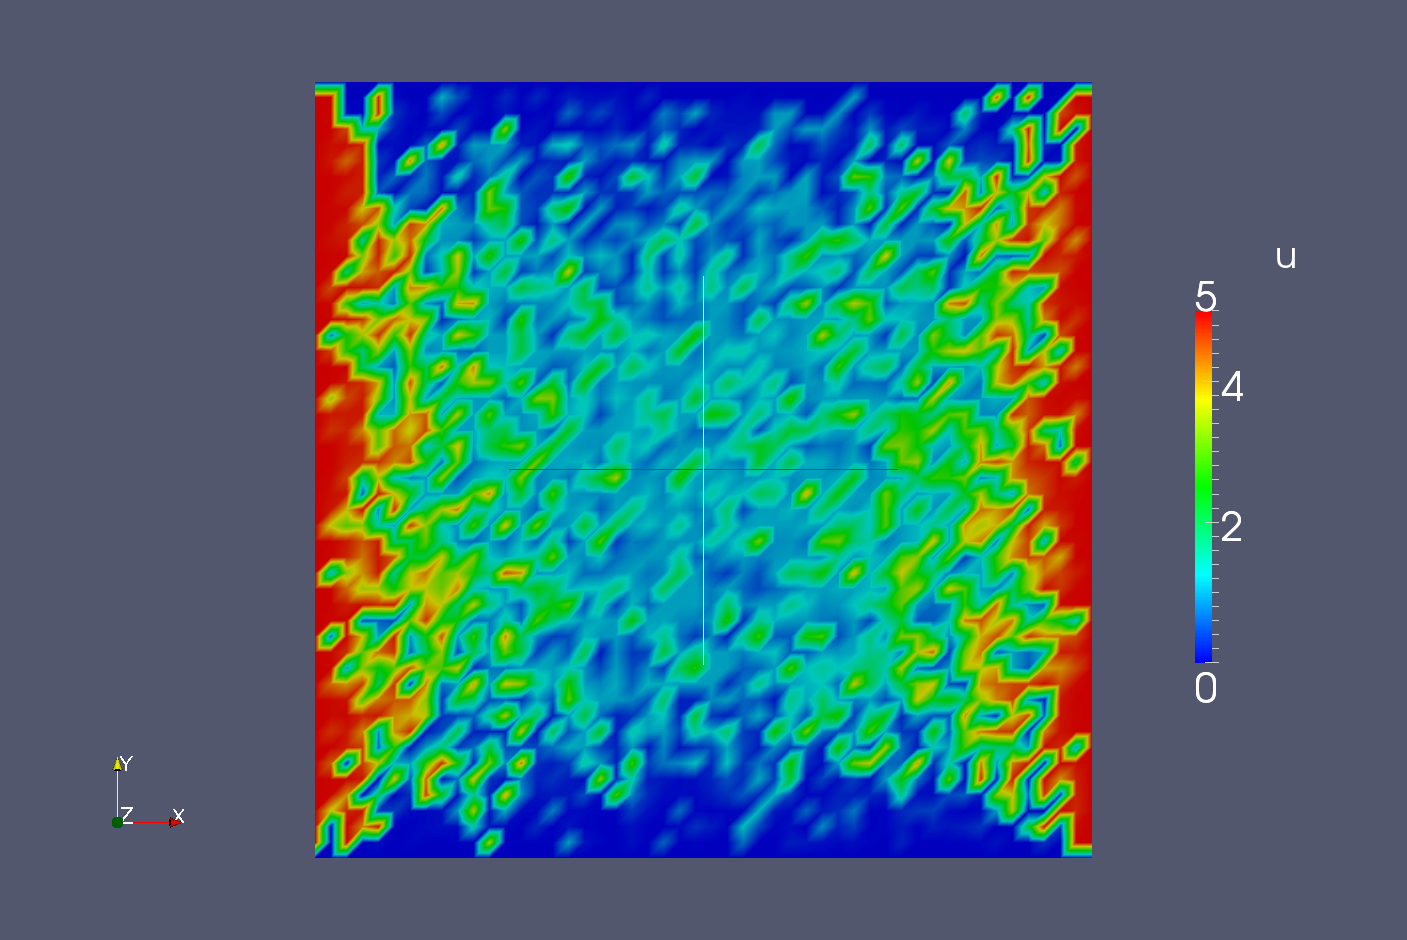
\includegraphics[width=4in]{direct_1.png}
    \end{center}
    \caption{\textbf{Direct solution to Poisson Equation.} \textit{1
        history per state, \sn{2.5}{3} total histories. 0.785 seconds
        CPU time.} }
  \end{figure}

\end{frame}

%%---------------------------------------------------------------------------%%
\begin{frame}{Direct Method: Evolution of a Solution}

  \begin{figure}[h!]
    \begin{center}
      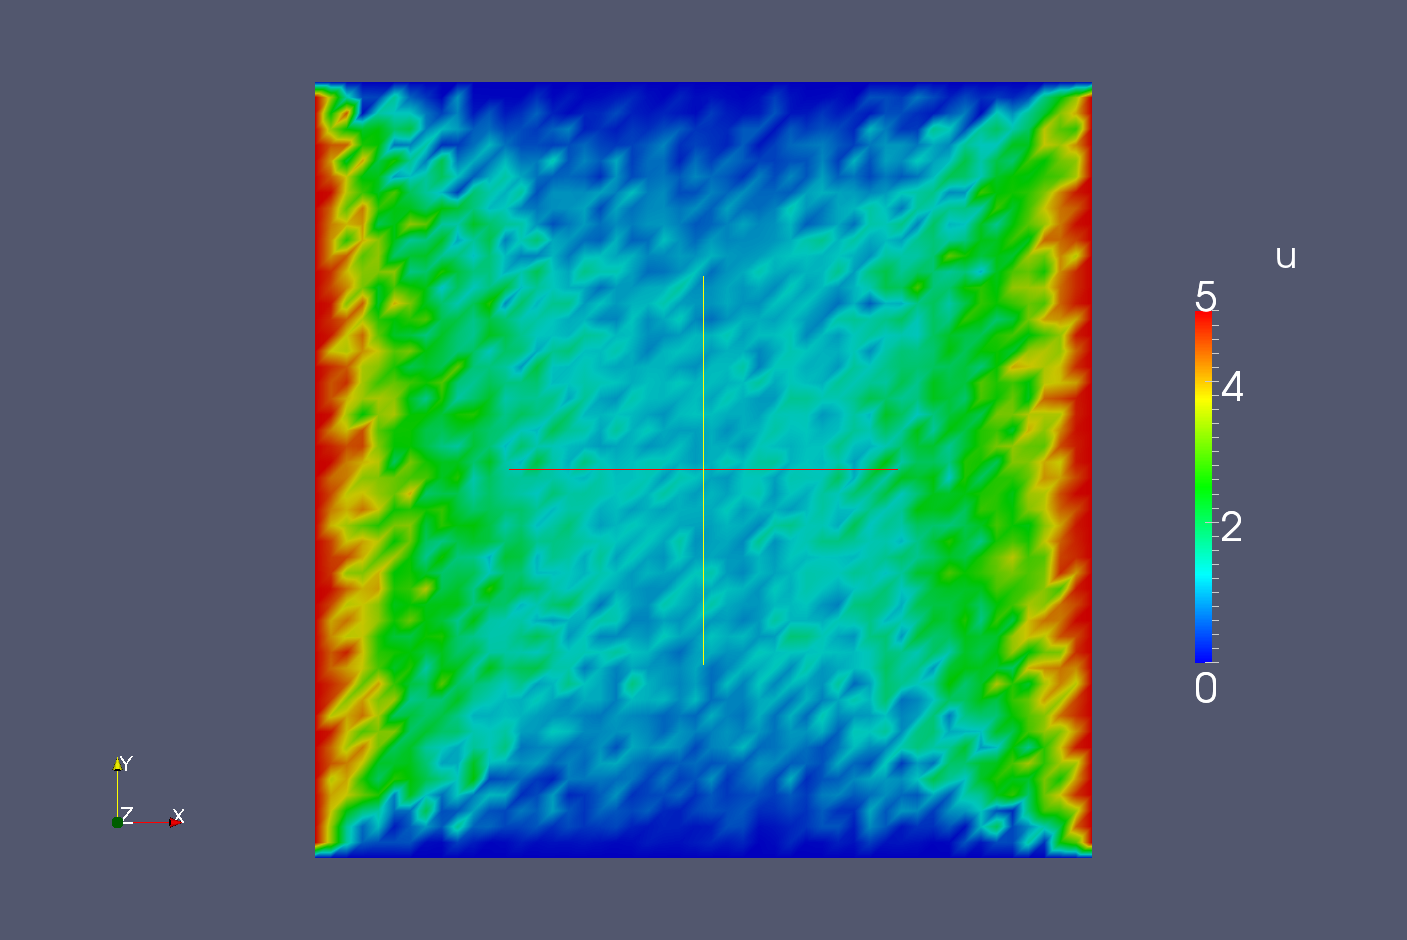
\includegraphics[width=4in]{direct_10.png}
    \end{center}
    \caption{\textbf{Direct solution to Poisson Equation.} \textit{10
        histories per state, \sn{2.5}{4} total histories. 5.9 seconds
        CPU time.} }
  \end{figure}

\end{frame}

%%---------------------------------------------------------------------------%%
\begin{frame}{Direct Method: Evolution of a Solution}

  \begin{figure}[h!]
    \begin{center}
      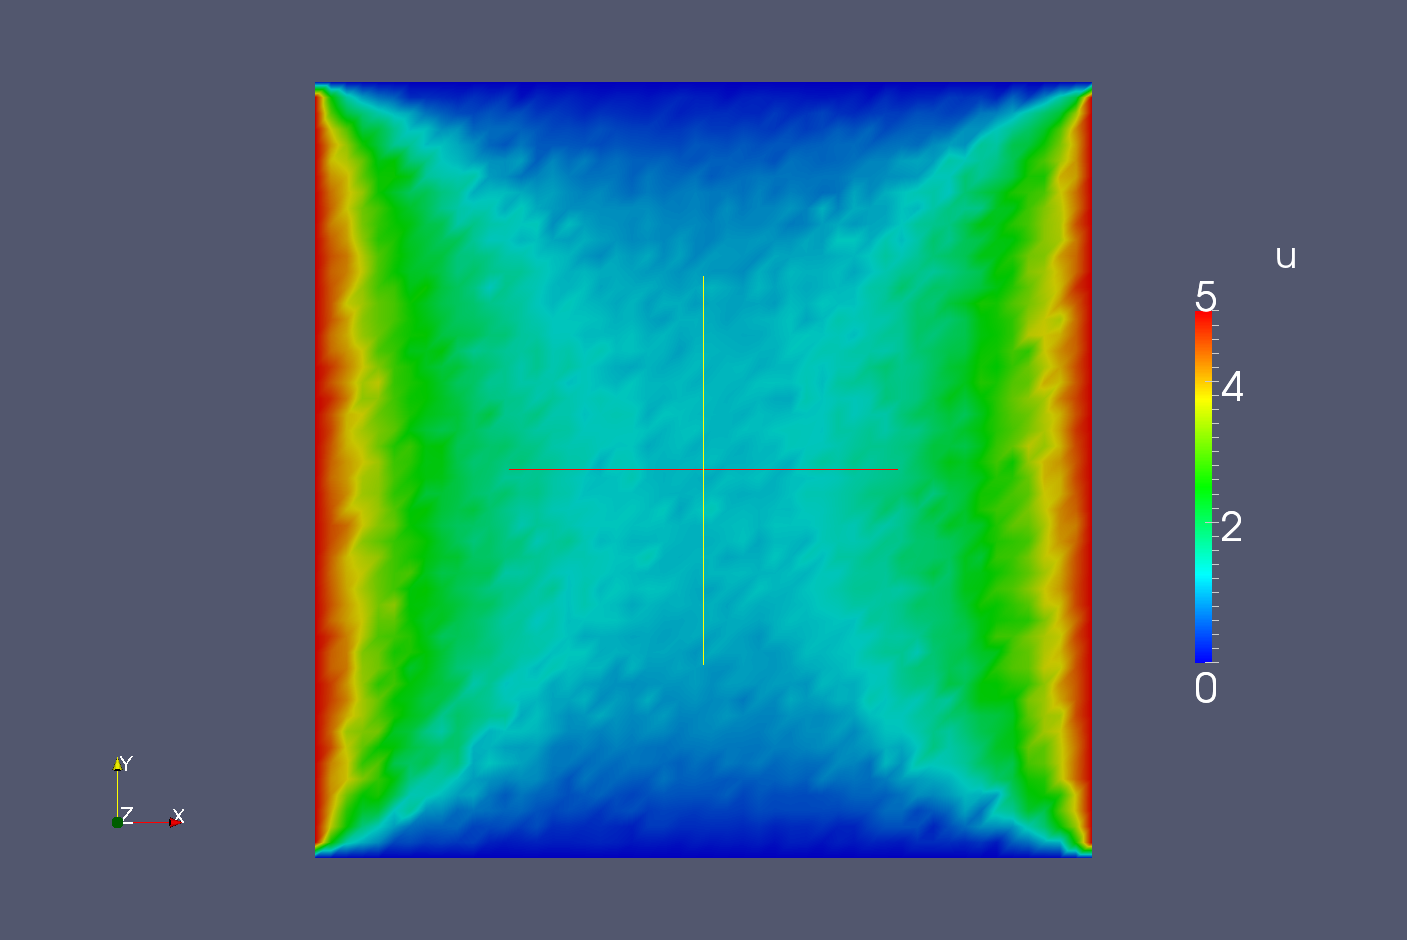
\includegraphics[width=4in]{direct_100.png}
    \end{center}
    \caption{\textbf{Direct solution to Poisson Equation.}
      \textit{100 histories per state, \sn{2.5}{5} total
        histories. 54.7 seconds CPU time.} }
  \end{figure}

\end{frame}

%%---------------------------------------------------------------------------%%
\begin{frame}{Direct Method: Evolution of a Solution}

  \begin{figure}[h!]
    \begin{center}
      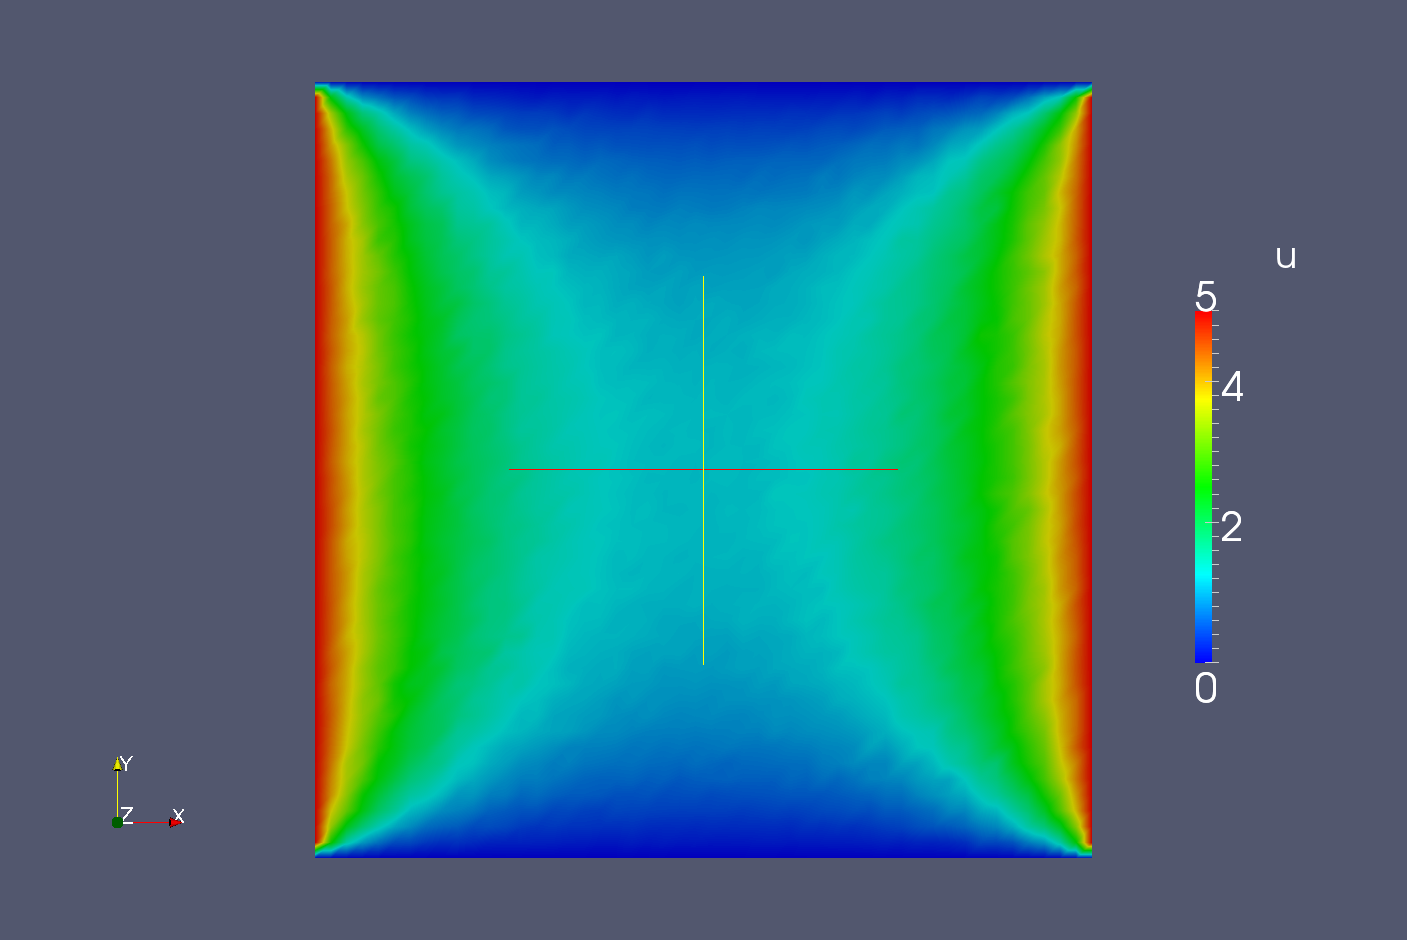
\includegraphics[width=4in]{direct_1000.png}
    \end{center}
    \caption{\textbf{Direct solution to Poisson Equation.} \textit{1000
        histories per state, \sn{2.5}{6} total histories. 644 seconds
        CPU time.} }
  \end{figure}

\end{frame}

%%---------------------------------------------------------------------------%%
\begin{frame}{Adjoint Method}

  \begin{itemize}
  \item Solve the adjoint linear system
  \end{itemize}

  \[
  \ve{A}^T \ve{y} = \ve{d}
  \]

  \[
  \ve{y} = \ve{H}^T \ve{y} + \ve{d}
  \]

  \begin{itemize}
  \item Set the adjoint constraint
  \end{itemize}

  \[
  \langle \ve{A}^T \ve{x}, \ve{y} \rangle = \langle \ve{x}, \ve{A}
  \ve{y} \rangle
  \]

  \[
  \langle \ve{x}, \ve{d} \rangle = \langle \ve{y}, \ve{b} \rangle
  \]
  
\end{frame}

%%---------------------------------------------------------------------------%%
\begin{frame}{Adjoint Method}

  \begin{itemize}
  \item Generate the Neumann series for the adjoint operator
  \end{itemize}

  \[
  \ve{y} = (\ve{I} - \ve{H}^T)^{-1} \ve{d}
  \]

  \[
  \ve{y} = \sum_{k=0}^{\infty} (\ve{H}^T)^k\ve{d}
  \]

  \begin{itemize}
  \item Expand the series
  \end{itemize}

  \[
  y_i = \sum_{k=0}^{\infty}\sum_{i_1}^{N}\sum_{i_2}^{N}\ldots
  \sum_{i_k}^{N}h_{i_k,i_{k-1}}\ldots h_{i_2,i_1} h_{i_1,i} d_{i_k}
  \]

  \begin{itemize}
  \item Pick another constraint to yield the original solution
  \end{itemize}

  \[
  \ve{d} = \boldsymbol{\delta}_i,\ \langle \ve{y}, \ve{b} \rangle =
  \langle \ve{x}, \boldsymbol{\delta}_i \rangle = x_i
  \]
  
\end{frame}

%%---------------------------------------------------------------------------%%
\begin{frame}{Adjoint Method}

  \begin{itemize}
  \item Use the adjoint Neumann-Ulam decomposition
  \end{itemize}

  \[
  \ve{H}^{T} = \ve{P} \circ \ve{W}
  \]

  \[
  p_{ij} = \frac{|h_{ji}|}{\sum_j |h_{ji}|},\ w_{ij} =
  \frac{h_{ji}}{p_{ij}}
  \]

  \begin{itemize}
  \item Build the estimator and expectation value
  \end{itemize}

  \[
  X_{\nu} = \sum_{m=0}^k W_{m} \delta_{i,i_m}
  \]

  \[
  \begin{split}
    E\{X_j\} &=\sum_{k=0}^{\infty}\sum_{i_1}^{N}\sum_{i_2}^{N}\ldots
    \sum_{i_k}^{N} b_{i_0} h_{i_0,i_1}h_{i_1,i_2}\ldots h_{i_{k-1},i_k}
    \delta_{i_k,j} \\ &= x_{j}
  \end{split}
  \]

\end{frame}

%%---------------------------------------------------------------------------%%
\begin{frame}{Adjoint Method: Evolution of a Solution}

  \begin{figure}[h!]
    \begin{center}
      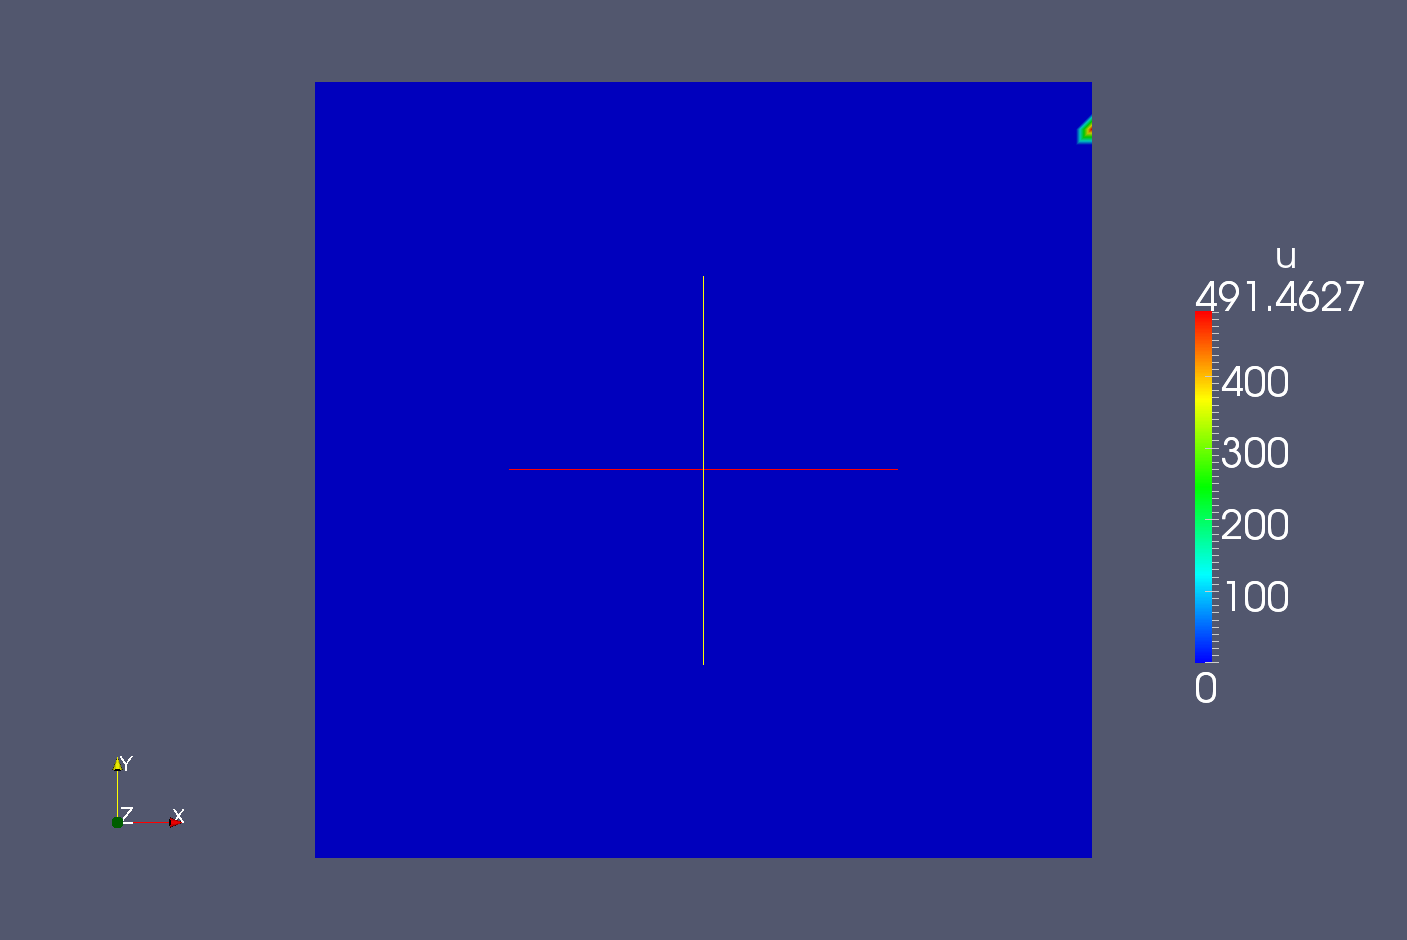
\includegraphics[width=4in]{adjoint_1.png}
    \end{center}
    \caption{\textbf{Adjoint solution to Poisson Equation.}
      \textit{\sn{1}{0} total histories, 0.286 seconds CPU time.} }
  \end{figure}

\end{frame}

%%---------------------------------------------------------------------------%%
\begin{frame}{Adjoint Method: Evolution of a Solution}

  \begin{figure}[h!]
    \begin{center}
      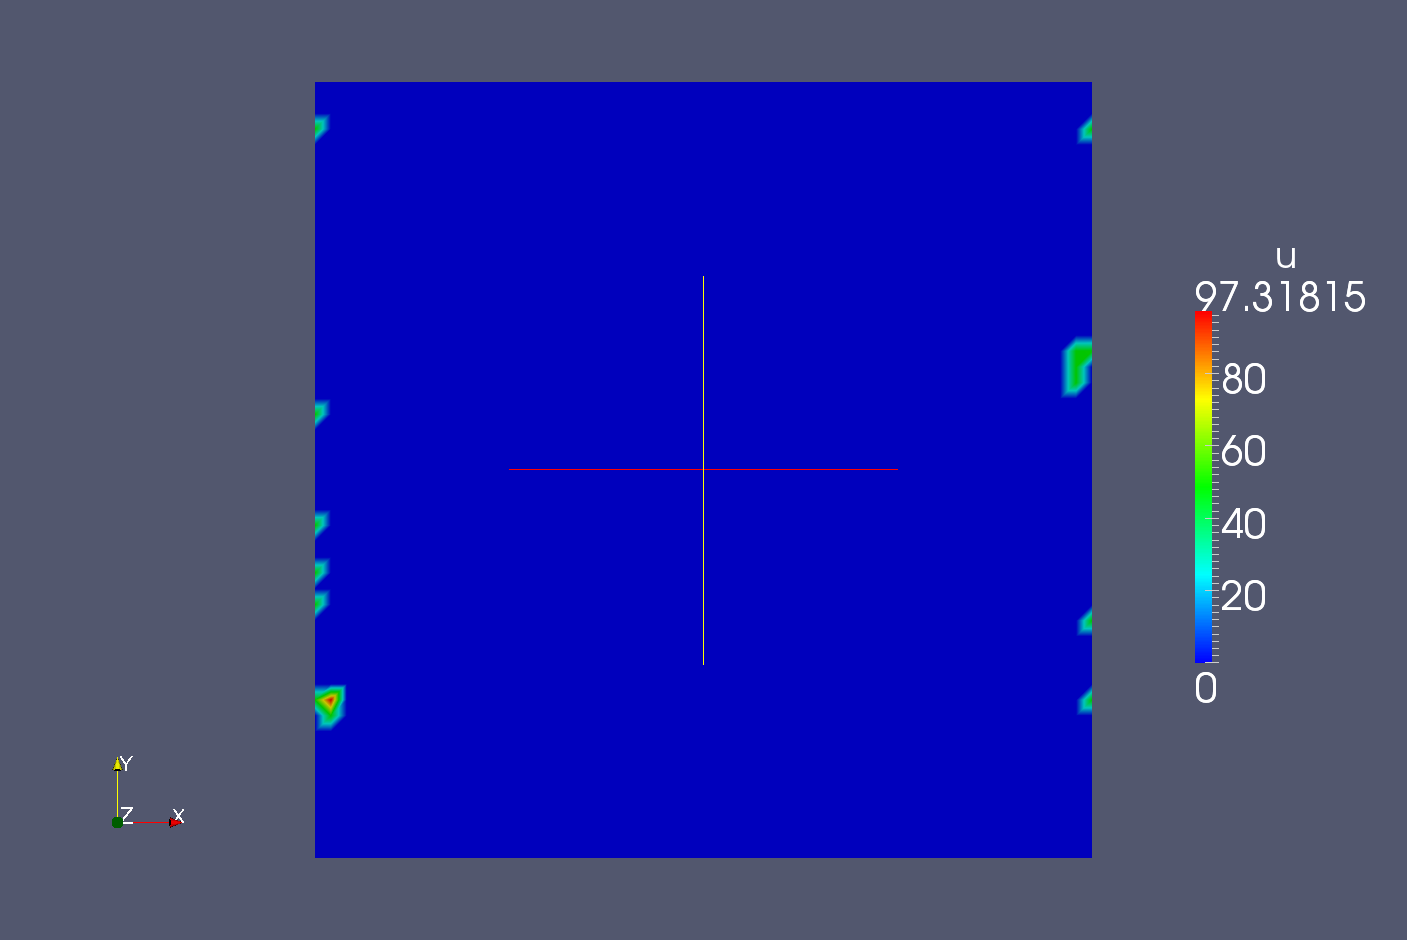
\includegraphics[width=4in]{adjoint_10.png}
    \end{center}
    \caption{\textbf{Adjoint solution to Poisson Equation.}
      \textit{\sn{1}{1} total histories, 0.278 seconds CPU time.} }
  \end{figure}

\end{frame}

%%---------------------------------------------------------------------------%%
\begin{frame}{Adjoint Method: Evolution of a Solution}

  \begin{figure}[h!]
    \begin{center}
      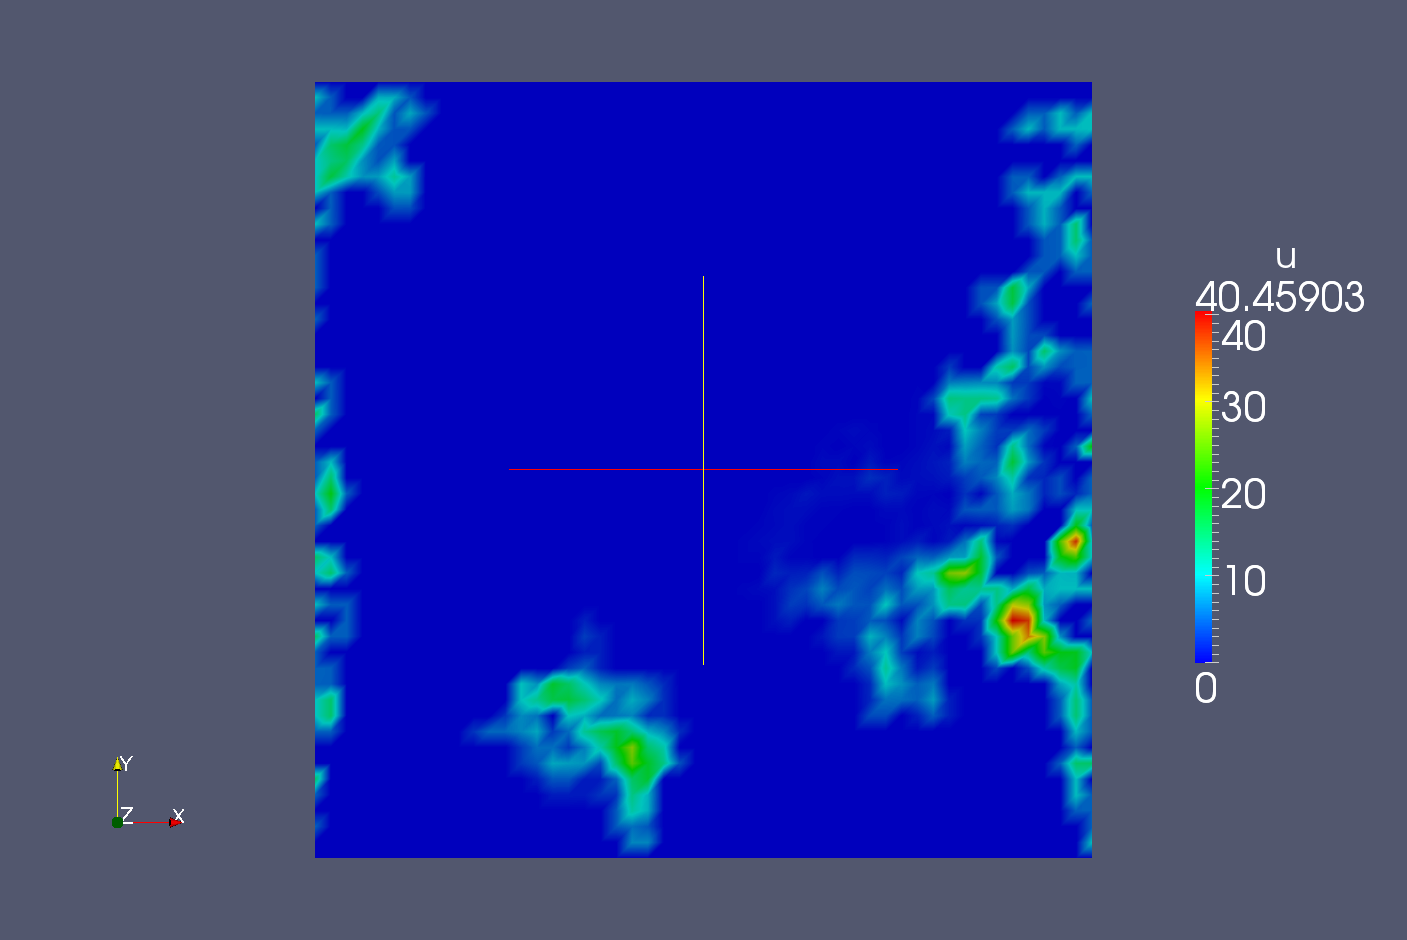
\includegraphics[width=4in]{adjoint_100.png}
    \end{center}
    \caption{\textbf{Adjoint solution to Poisson Equation.}
      \textit{\sn{1}{2} total histories, 0.275 seconds CPU time.} }
  \end{figure}

\end{frame}

%%---------------------------------------------------------------------------%%
\begin{frame}{Adjoint Method: Evolution of a Solution}

  \begin{figure}[h!]
    \begin{center}
      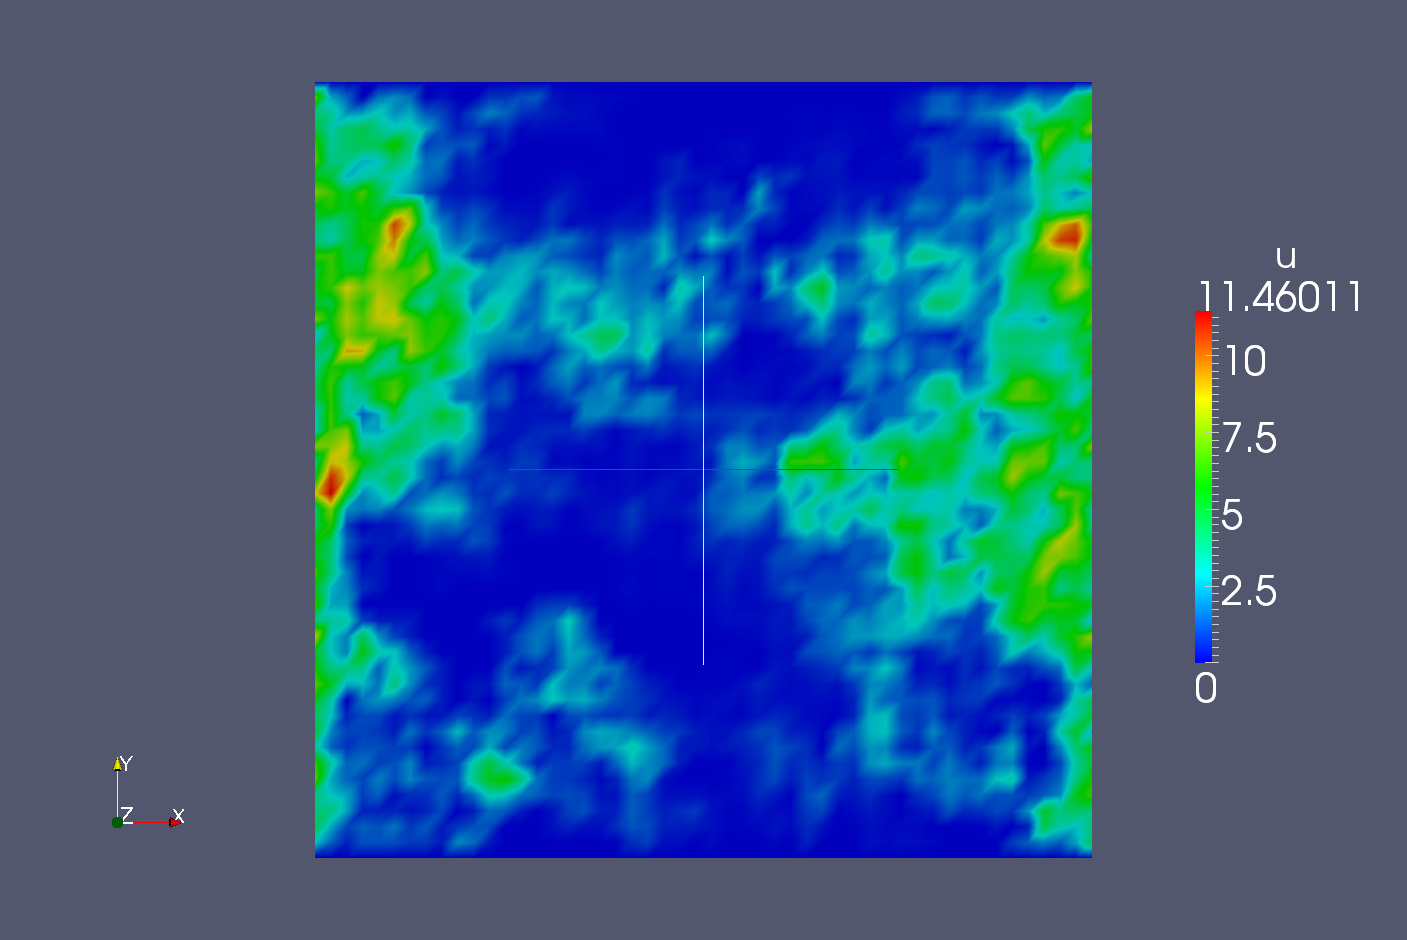
\includegraphics[width=4in]{adjoint_1000.png}
    \end{center}
    \caption{\textbf{Adjoint solution to Poisson Equation.}
      \textit{\sn{1}{3} total histories, 0.291 seconds CPU time.} }
  \end{figure}

\end{frame}

%%---------------------------------------------------------------------------%%
\begin{frame}{Adjoint Method: Evolution of a Solution}

  \begin{figure}[h!]
    \begin{center}
      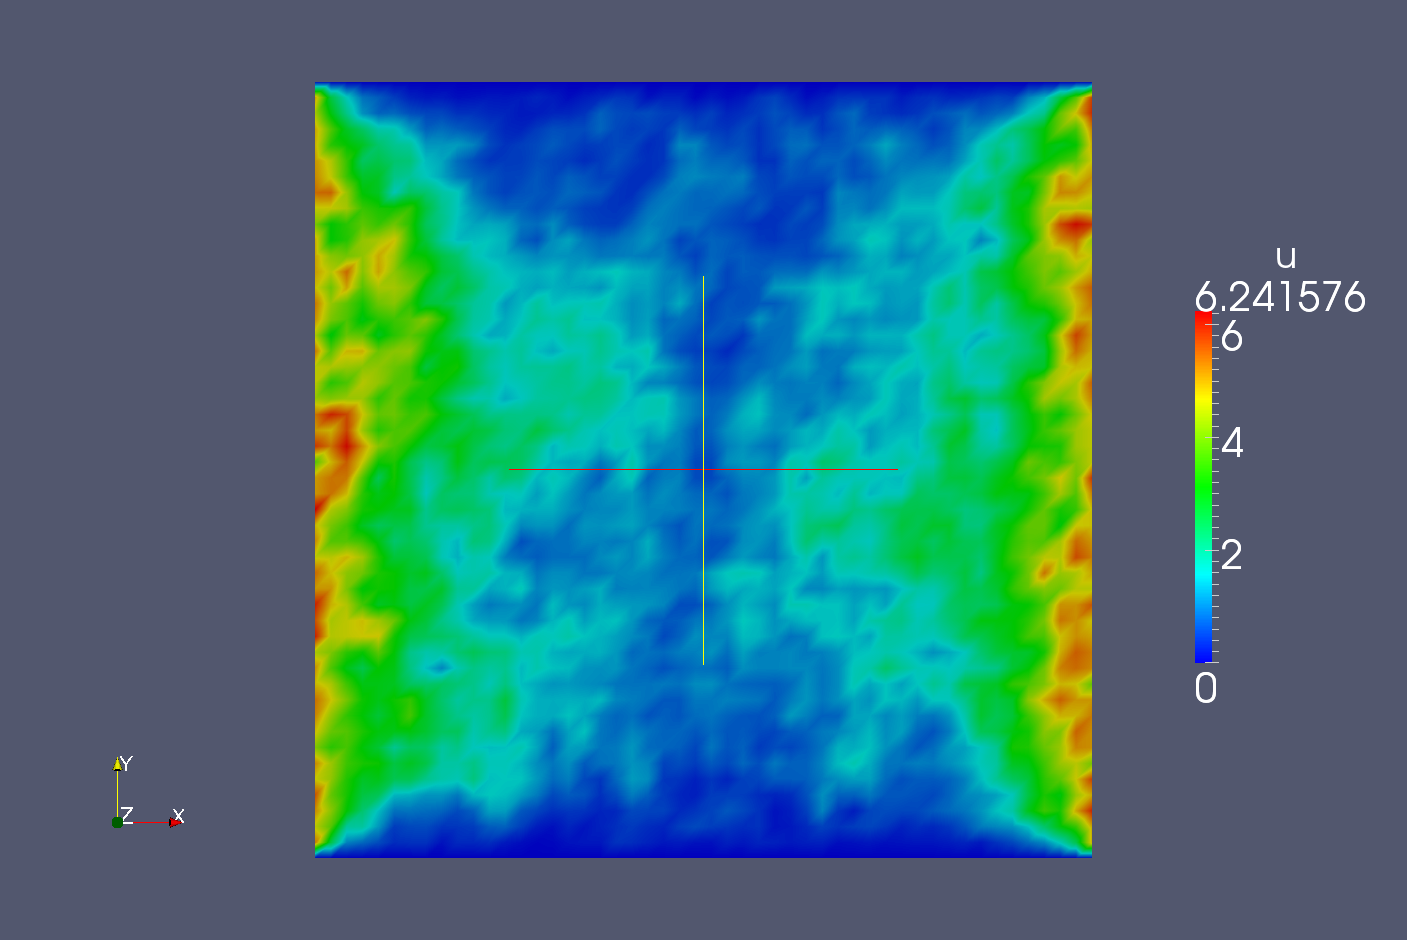
\includegraphics[width=4in]{adjoint_10000.png}
    \end{center}
    \caption{\textbf{Adjoint solution to Poisson Equation.}
      \textit{\sn{1}{4} total histories, 0.428 seconds CPU time.} }
  \end{figure}

\end{frame}

%%---------------------------------------------------------------------------%%
\begin{frame}{Adjoint Method: Evolution of a Solution}

  \begin{figure}[h!]
    \begin{center}
      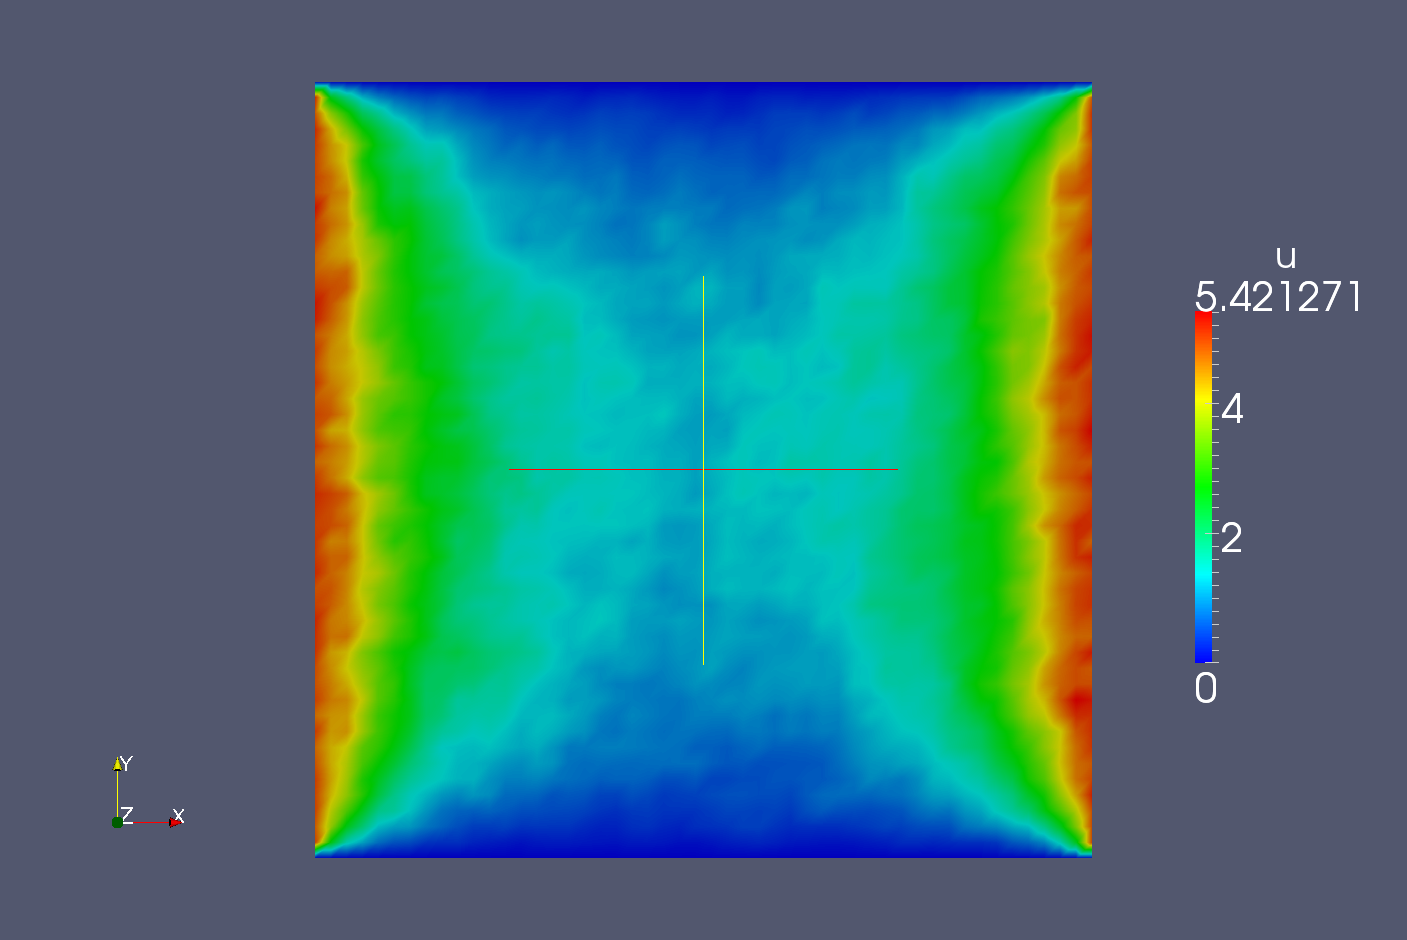
\includegraphics[width=4in]{adjoint_100000.png}
    \end{center}
    \caption{\textbf{Adjoint solution to Poisson Equation.}
      \textit{\sn{1}{5} total histories, 1.76 seconds CPU time.} }
  \end{figure}

\end{frame}

%%---------------------------------------------------------------------------%%
\begin{frame}{Adjoint Method: Evolution of a Solution}

  \begin{figure}[h!]
    \begin{center}
      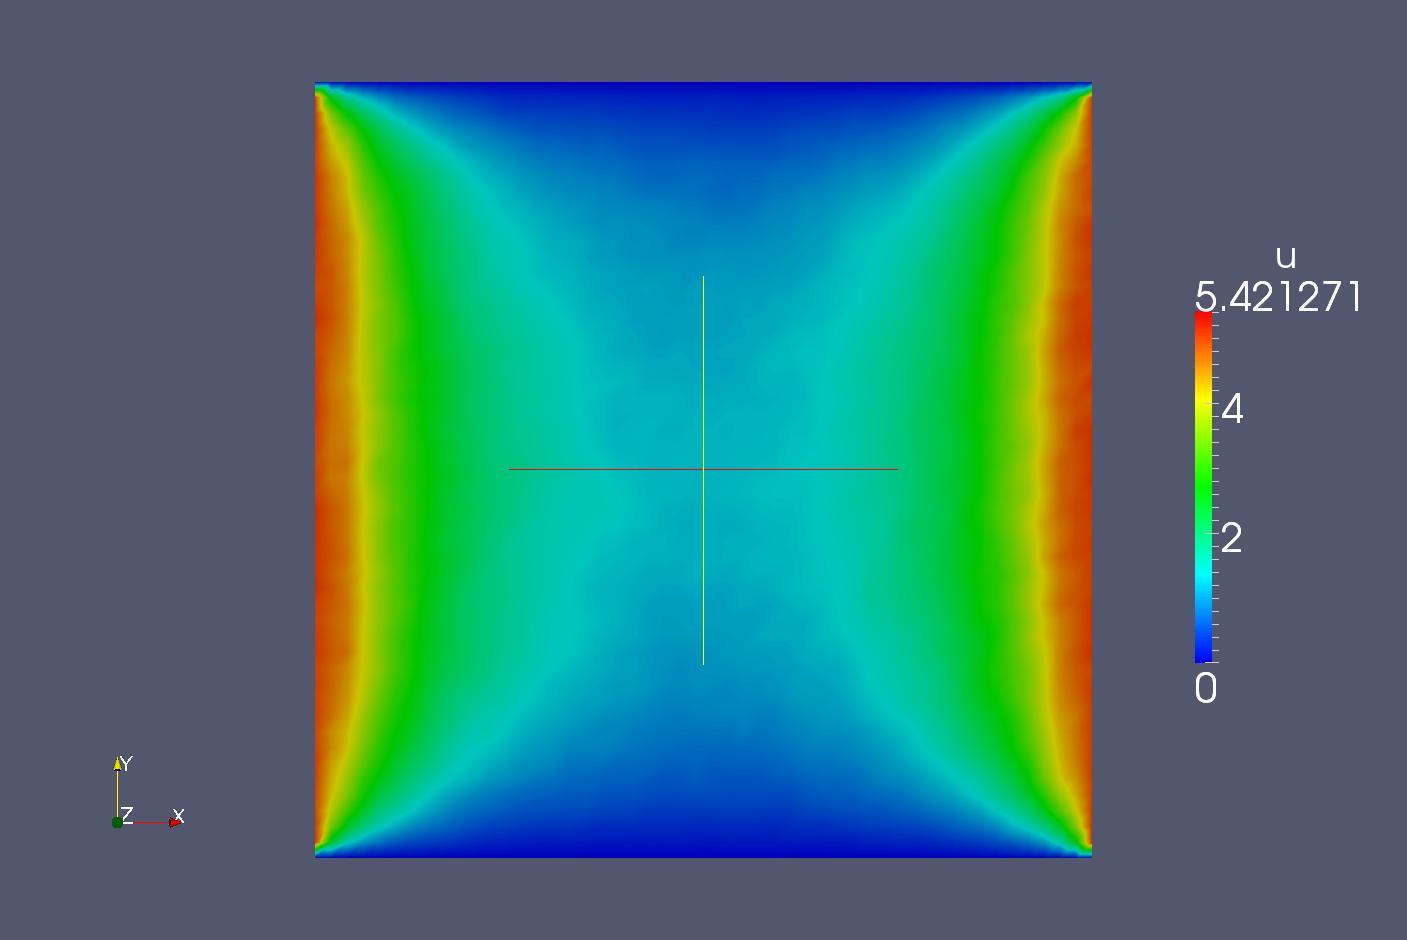
\includegraphics[width=4in]{adjoint_1000000.png}
    \end{center}
    \caption{\textbf{Adjoint solution to Poisson Equation.}
      \textit{\sn{1}{6} total histories, 15.1 seconds CPU time.} }
  \end{figure}

\end{frame}

%%---------------------------------------------------------------------------%%
\begin{frame}{Adjoint Method: Evolution of a Solution}

  \begin{figure}[h!]
    \begin{center}
      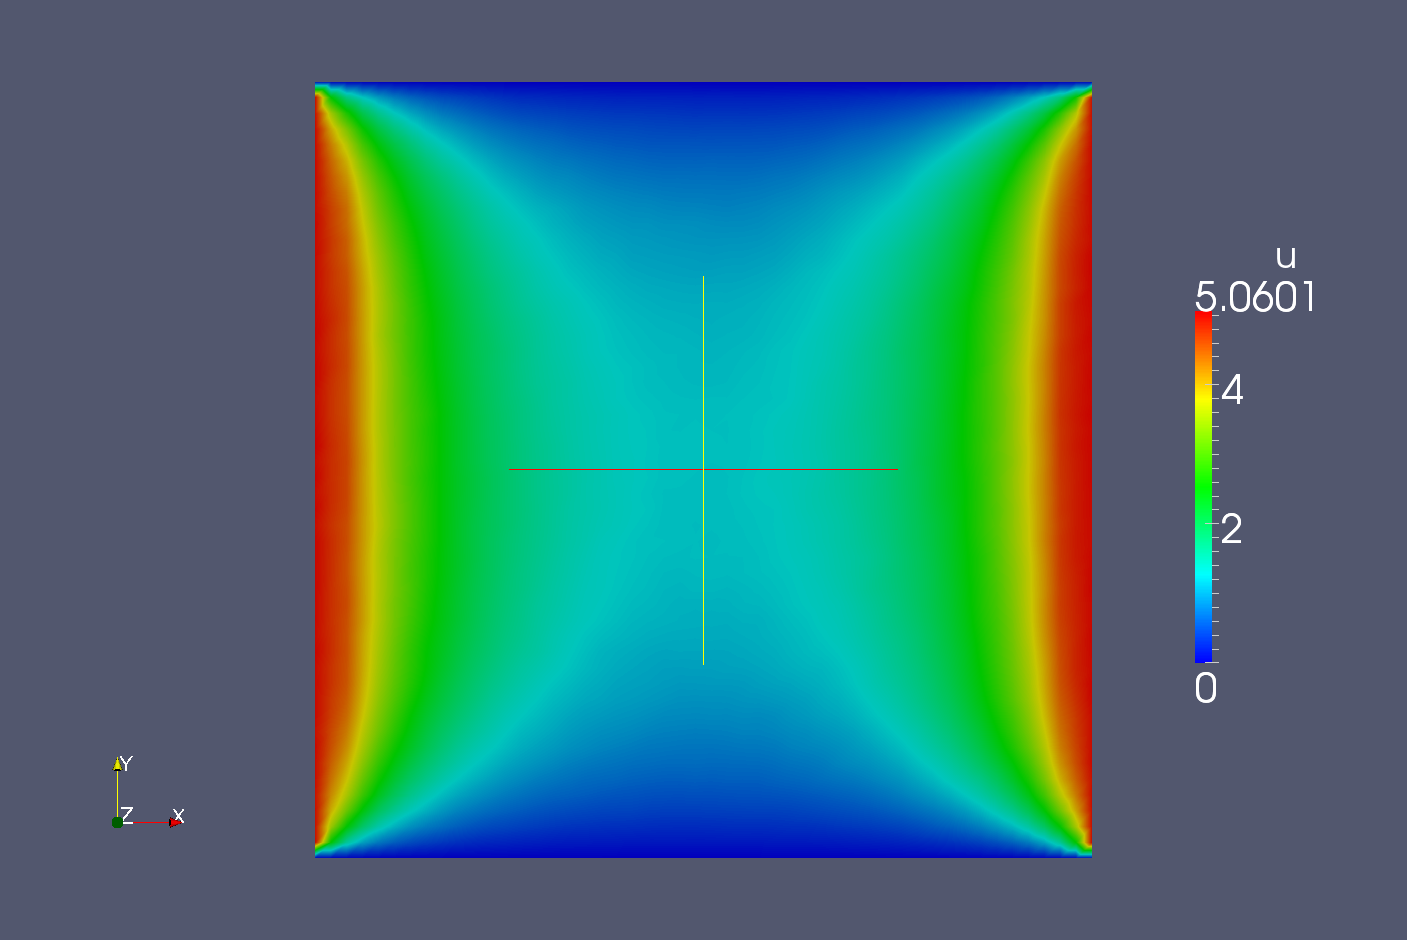
\includegraphics[width=4in]{adjoint_10000000.png}
    \end{center}
    \caption{\textbf{Adjoint solution to Poisson Equation.}
      \textit{\sn{1}{7} total histories, 149 seconds CPU time.} }
  \end{figure}

\end{frame}

%%---------------------------------------------------------------------------%%
\begin{frame}{Sequential Monte Carlo}

  \begin{itemize}
  \item Neumann-Ulam methods bound by the Central Limit Theorem
  \item Halton proposed an iterative residual method in 1962
  \item Iteration error decoupled from Monte Carlo error
  \item Exponential convergence (Evans,2003)
  \end{itemize}

  \[
  \ve{r}^k = \ve{b} - \ve{A}\ve{x}^k
  \]
  \[
  \ve{A}\boldsymbol{\delta}^{k} = \ve{r}^{k}
  \]
  \[
  \ve{x}^{k+1} = \ve{x}^k + \boldsymbol{\delta}^{k}
  \]

\end{frame}

%%---------------------------------------------------------------------------%%
\begin{frame}{Monte Carlo Synthetic-Acceleration}

  \begin{beamerboxesrounded}[upper=boxheadcolor,lower=boxbodycolor,shadow=true]
    {MCSA Iteration (Evans,2009)}

    \[
    \ve{x}^{k+1/2} = (\ve{I} - \ve{A})\ve{x}^k + \ve{b}
    \]
    \[
    \ve{r}^{k+1/2} = \ve{b} - \ve{A}\ve{x}^{k+1/2}
    \]
    \[
    \hat{\ve{A}}\delta\ve{x}^{k+1/2} = \ve{r}^{k+1/2}
    \]
    \[
    \ve{x}^{k+1} = \ve{x}^{k+1/2} + \delta \ve{x}^{k+1/2}
    \]

  \end{beamerboxesrounded}

  \begin{itemize}
  \item Adjoint Neumann-Ulam solver computes the correction
  \item Decouples Monte Carlo error from solution error
  \item Exponential convergence
  \item Demonstrated by Evans and colleagues to be competitive with
    Krylov methods
  \end{itemize}

\end{frame}

%%---------------------------------------------------------------------------%%
\begin{frame}{Preconditioning Monte Carlo Methods}

  \begin{itemize}
  \item No symmetry requirements
  \item Require $\rho(\ve{H}) < 1$
  \item Choose Jacobi preconditioning at a minimum
  \end{itemize}

  \[
  \ve{M} = diag(\ve{A})
  \]
  \[
  \ve{M}^{-1}\ve{A}\ve{x} = \ve{M}^{-1}\ve{b}
  \]
  
  \begin{itemize}
  \item Yields a preconditioned MCSA iteration with no in-state
    transitions
  \end{itemize}

  \[
  \ve{x}^{k+1/2} = (\ve{I} - \ve{M}^{-1}\ve{A})\ve{x}^k + \ve{b}
  \]
  \[
  \ve{r}^{k+1/2} = \ve{b} - \ve{M}^{-1}\ve{A}\ve{x}^{k+1/2}
  \]
  \[
  \ve{M}^{-1}\ve{A}\delta\ve{x}^{k+1/2} = \ve{r}^{k+1/2}
  \]
  \[
  \ve{x}^{k+1} = \ve{x}^{k+1/2} + \delta \ve{x}^{k+1/2}
  \]

\end{frame}

%%---------------------------------------------------------------------------%%
\begin{frame}{Direct vs. Adjoint Analysis}

  \begin{itemize}
  \item Analysis needed to select Monte Carlo method
  \item Time-dependent 2-dimensional Poisson equation
  \item Spectral radius fixed
  \item Sparsity varied with 2 Laplacian stencils
  \end{itemize}

  \[
  \nabla^2_5 = \frac{1}{\Delta^2}[u_{i-1,j} + u_{i+1,j} + u_{i,j-1} +
    u_{i,j+1} - 4 u_{i,j}]
  \]
  \[
  \begin{split}
    \nabla^2_9 = \frac{1}{6\Delta^2}[4 u_{i-1,j} + 4 u_{i+1,j} + 4
      u_{i,j-1} + 4 u_{i,j+1} + u_{i-1,j-1}\\ + u_{i-1,j+1} +
      u_{i+1,j-1} + u_{i+1,j+1} - 20 u_{i,j}]
  \end{split}
  \]

  \begin{itemize}
  \item Implicit Euler time differencing
  \end{itemize}

  \[
  \ve{A} \ve{u}^{n+1} = \ve{u}^n
  \]

\end{frame}

%%---------------------------------------------------------------------------%%
\begin{frame}{Direct vs. Adjoint Analysis}

  \begin{columns}

    \begin{column}{0.5\textwidth}
      \begin{figure}[h!]
        \centering
        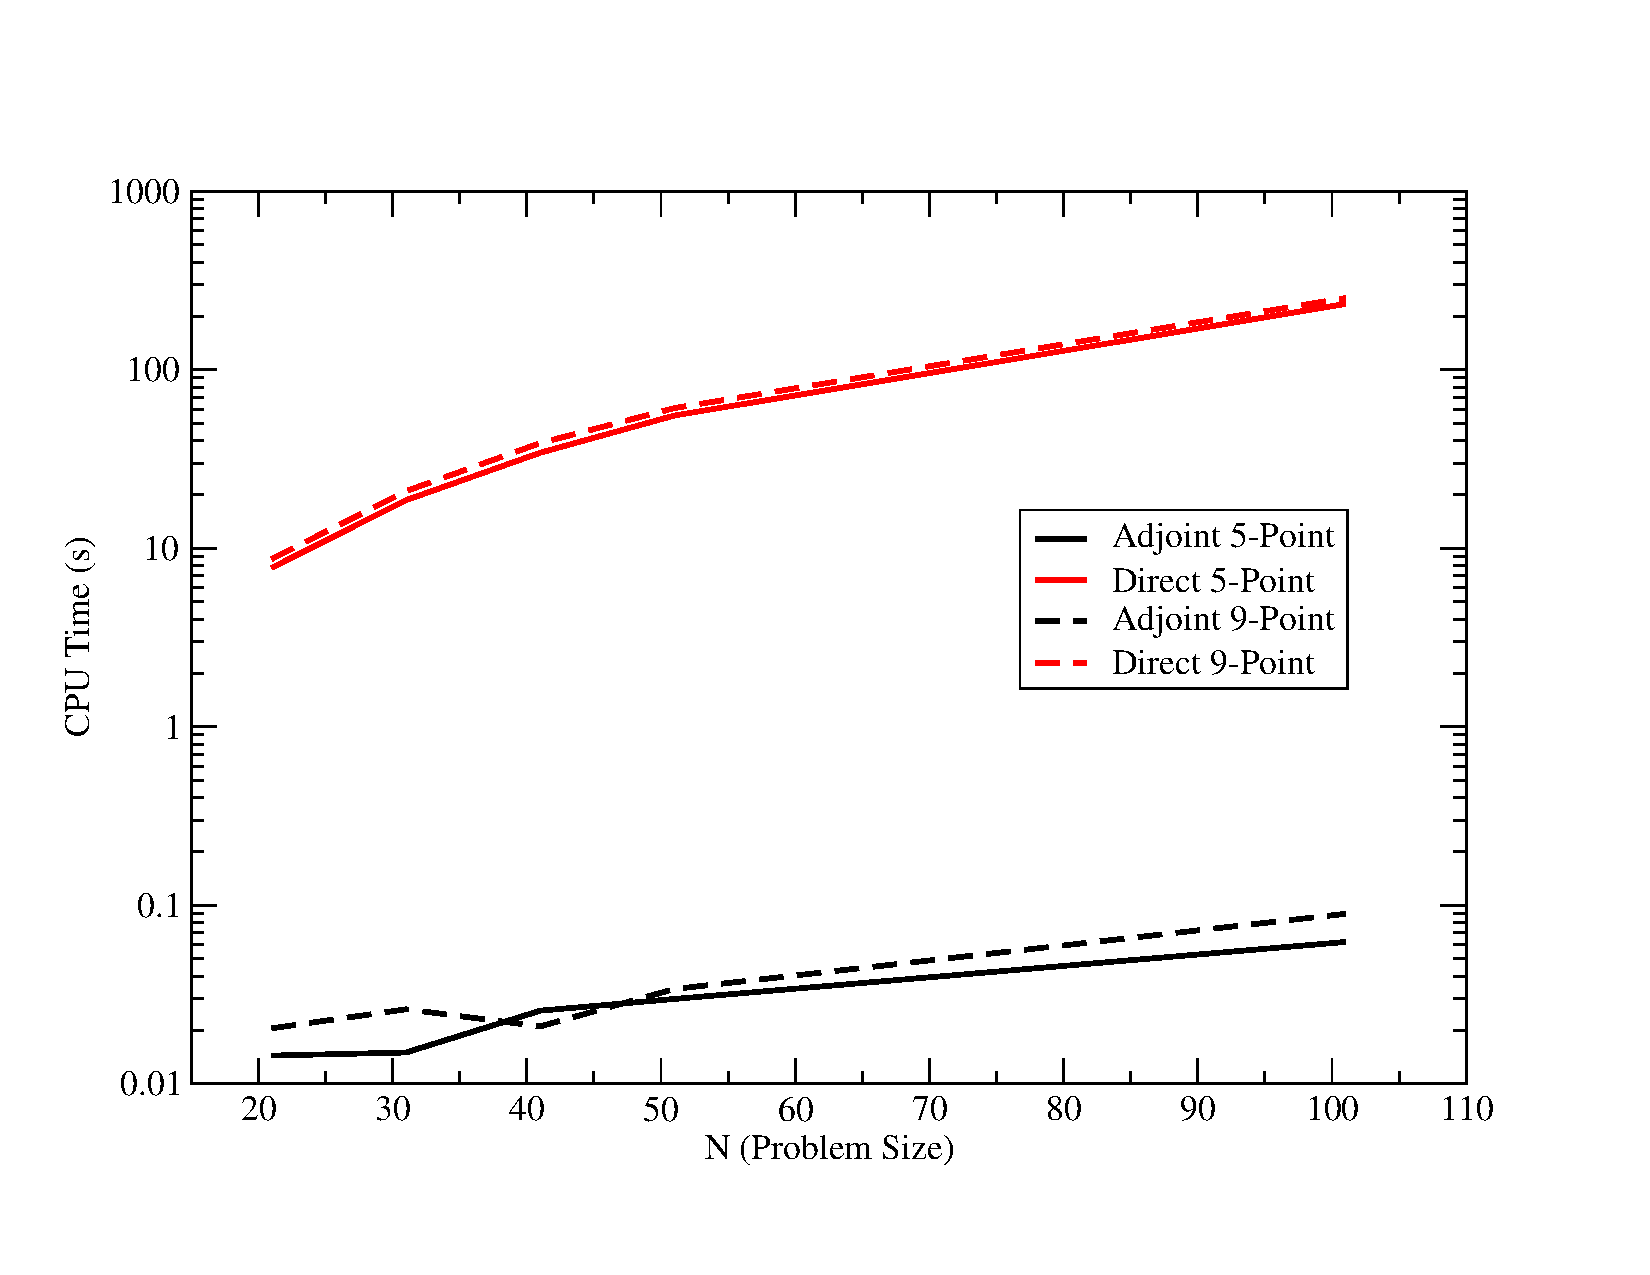
\includegraphics[width=2.5in,clip]{Adjoint_Direct_CPU_Time.pdf}
        \caption{\textbf{CPU Time (s) to converge vs. Problem Size
            ($N$ for an $N \times N$ square mesh).} }
      \end{figure}
    \end{column}

    \begin{column}{0.5\textwidth}
      \begin{figure}[h!]
        \centering
        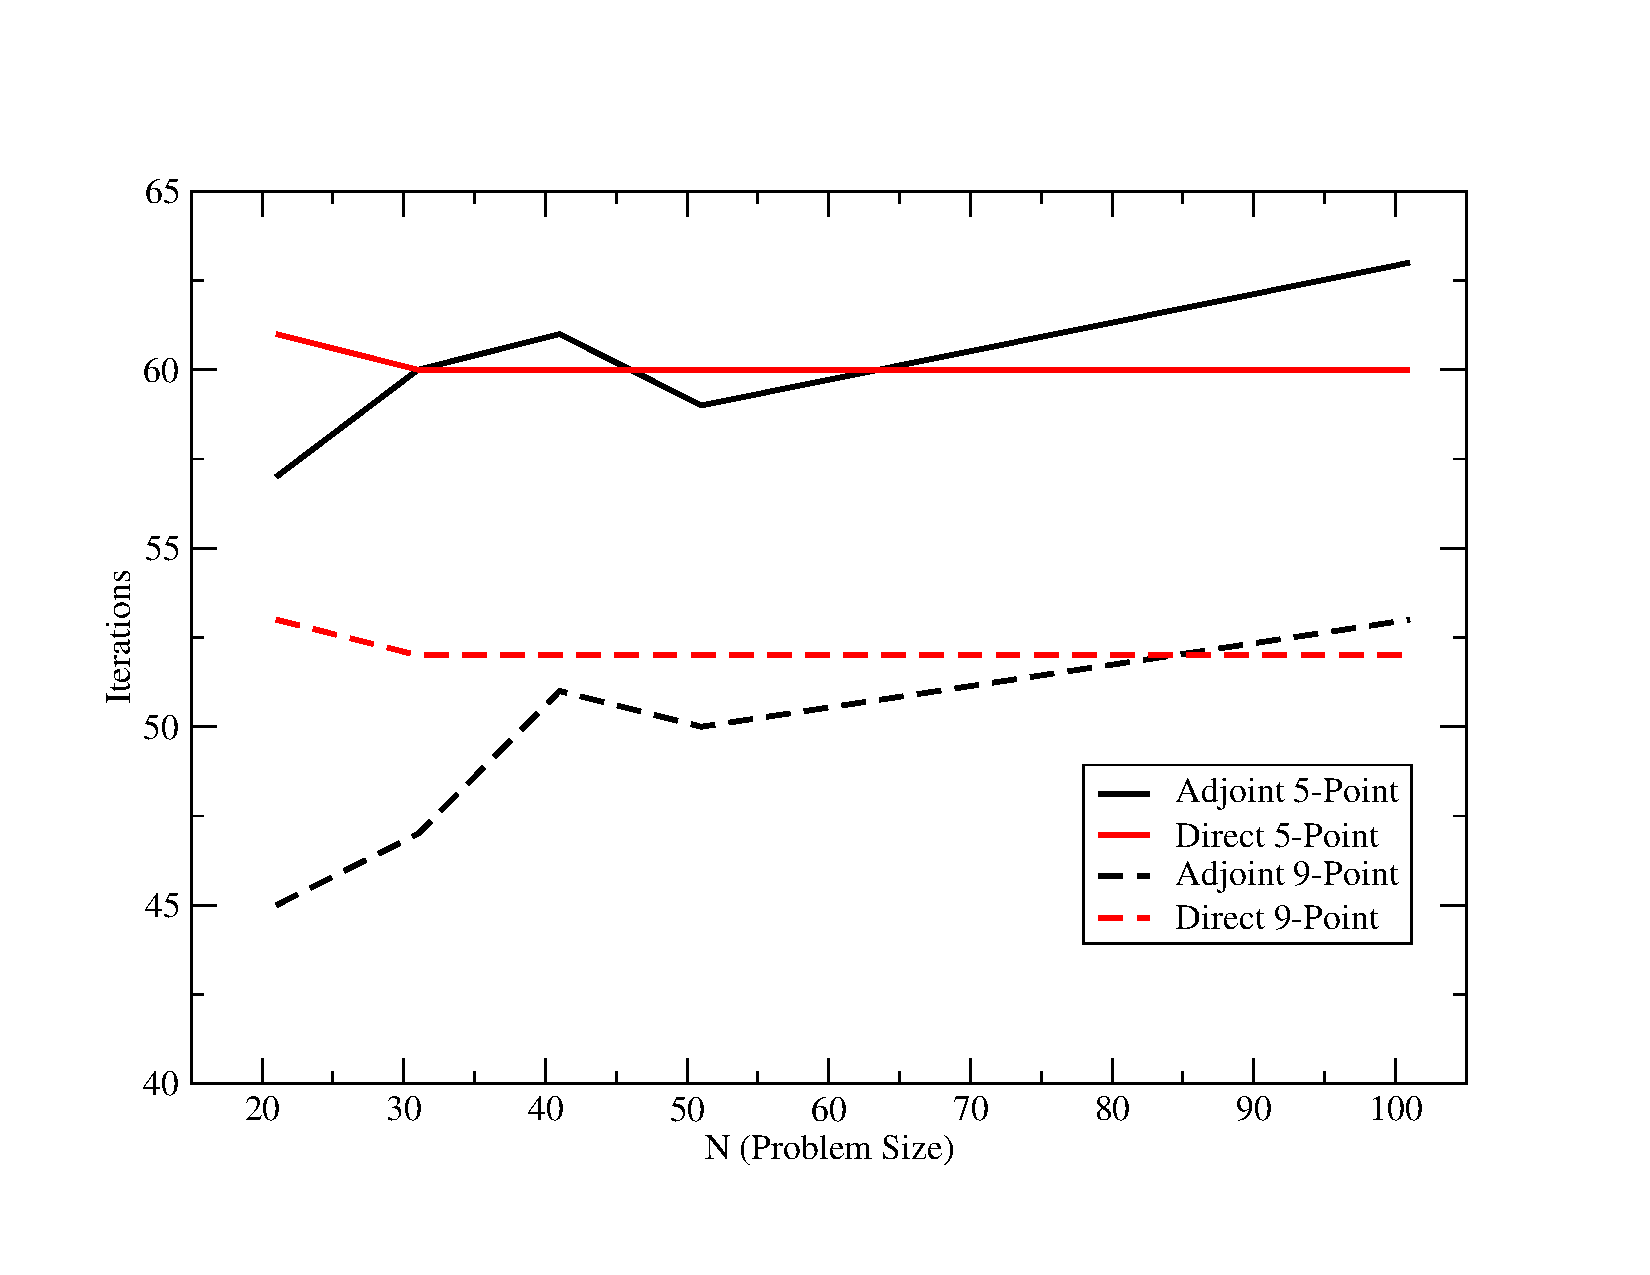
\includegraphics[width=2.5in,clip]{Adjoint_Direct_Iterations.pdf}
        \caption{\textbf{Iterations to converge vs. Problem Size ($N$
            for an $N \times N$ square mesh).} }
      \end{figure}
    \end{column}

  \end{columns}

\end{frame}

%%---------------------------------------------------------------------------%%
\begin{frame}{Direct vs. Adjoint Analysis}

  \begin{figure}[h!]
    \centering
    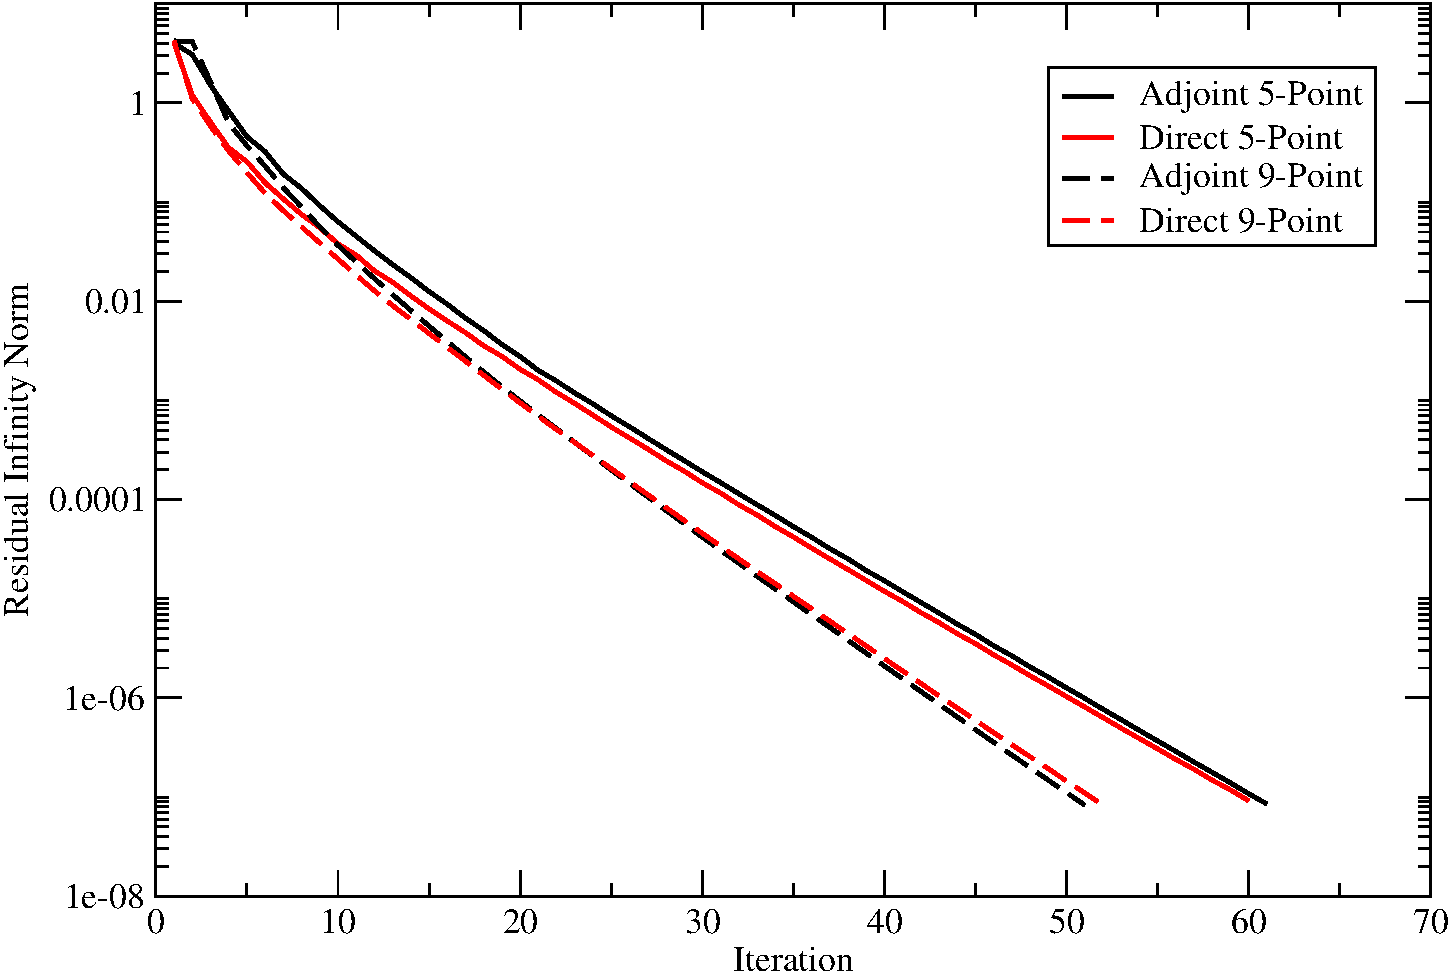
\includegraphics[width=2.5in,clip]{Adjoint_Direct_Convergence.pdf}
    \caption{\textbf{Infinity norm of the solution residual
        vs. iteration number for a problem of fixed size.} }
  \end{figure}

  \begin{itemize}
  \item CPU time dominating factor in method selection
  \item Significant speedup with adjoint method
  \item Does not affect convergence behavior
  \item Use adjoint with MCSA and Sequential Monte Carlo
  \end{itemize}

\end{frame}

%%---------------------------------------------------------------------------%%
\begin{frame}{Generalization of MCSA for Linear Problems}

  \begin{itemize}
  \item Published work to date has used a physics-based formulation
    \begin{itemize}
    \item Radiation transport equations used as model system
    \item Transition probabilities built from problem-specific
      parameters
    \item Probabilities and weights must be re-derived for each new
      equation set
    \end{itemize}
  \item Desire a generalization for all linear operator equations
    \begin{itemize}
    \item Requires a general parallel framework
    \item Requires implementation with a general linear algebra
      framework
    \item Operator, vector, and graph abstractions
    \end{itemize}
  \item Neumann-Ulam solvers and MCSA implemented using the Trilinos
    Petra frameworks
  \item Can be leveraged in modern physics implementations
  \end{itemize}

\end{frame}

%%---------------------------------------------------------------------------%%
\begin{frame}{Parallelization of Monte Carlo Methods}

  \begin{itemize}
  \item No literature observed for parallel Neumann-Ulam solvers
  \item Numerous references for modern parallel Monte Carlo methods in
    reactor physics
  \item Build a strategy for applying modern methods to the
    Neumann-Ulam method
  \item MCSA iteration-level parallelism comes from parallel
    matrix/vector operations
  \end{itemize}

\end{frame}

%%---------------------------------------------------------------------------%%
\begin{frame}{Domain Decomposition}

  \begin{itemize}
  \item Each parallel process owns a piece of the domain
  \item Random walks must be transported across domains through
    communication
  \end{itemize}

  \begin{beamerboxesrounded}[upper=boxheadcolor,lower=boxbodycolor,shadow=true]
    {Brunner's Work (2006 and 2009)}

    \begin{itemize}
    \item Looked at 4 communication patterns:
      \begin{itemize}
      \item Fully-locking synchronous
      \item asynchronous-send/synchronous-receive
      \item master/slave
      \item binary tree master/slave
      \end{itemize}
    \item Binary tree master/slave performed best but race conditions observed
    \item A later improvement to their work showed a fully asynchronous
      pattern to work best
    \item Poor scaling for unbalanced problems for all schemes
    \end{itemize}
    
  \end{beamerboxesrounded}

\end{frame}

%%---------------------------------------------------------------------------%%
\begin{frame}{Multiple-Set Overlapping-Domain Decomposition}

  \begin{columns}

    \begin{column}{0.5\textwidth}
      \begin{figure}[htpb!]
        \begin{center}
          \scalebox{0.75}{ \input{msod_example.pdftex_t} }
        \end{center}
        \caption{\textbf{Overlapping domain example illustrating how
            domain overlap can reduce communication costs.}}
      \end{figure}
    \end{column}

    \begin{column}{0.5\textwidth}
      \begin{itemize}
      \item Developed by Wagner and colleagues in 2010
      \item Each set contains the full domain
      \item Multiple sets replicate the domain
      \item Domains overlap within a set
      \item Reduces communication by a significant fraction
      \item Increases scalability through smaller processor sets
      \item Redundancy for resiliency (and useful work)
      \end{itemize}
    \end{column}

  \end{columns}

\end{frame}

%%---------------------------------------------------------------------------%%
\begin{frame}{Domain-to-Domain Communication}

  \begin{itemize}
  \item The amount of domain leakage dictates communication
  \item Per Siegel's 2012 work, define a leakage fraction
  \end{itemize}

  \[
  \lambda =
  \frac{average\ \#\ of\ particles\ leaving\ local\ domain}{total\ 
    of\ \#\ of\ particles\ starting\ in\ local\ domain}
  \]

  \begin{itemize}
  \item Siegel observed $\lambda$ to be bound empirically to the mean
    free path of the system
  \item Optimum ratio of local to global domain size exists
  \item Experiments show feasibility for large-scale calculations
    \begin{itemize}
    \item Not bandwidth or latency limited in load-balanced case
    \end{itemize}
    \pause
  \item How do we define $\lambda$ empirically for linear operator
    equations? 
  \end{itemize}

\end{frame}

%%---------------------------------------------------------------------------%%
\begin{frame}{Load Balancing}

  \begin{figure}[htpb!]
    \begin{center}
      \scalebox{1.0}{ \input{procassini_example.pdftex_t} }
    \end{center}
    \caption{\textbf{Example illustrating how domain decomposition can
        create load balance issues in Monte Carlo.}}
    \label{fig:procassini_example}
  \end{figure}

  \begin{itemize}
  \item Procassini's 2005 work addressed some concerns
  \item Dynamic balancing replicates domains independently
  \item Linear operator equations may benefit - fixed source problems
  \end{itemize}

\end{frame}

%%---------------------------------------------------------------------------%%
\begin{frame}{Parallel Adjoint Method}

Strategy
  \begin{itemize}
  \item Direct analogs between particle transport and Neumann-Ulam
    solvers 
  \item Aim for MSOD implementation and fully asynchronous
    communication patterns
  \end{itemize}

Questions
  \begin{itemize}
  \item How much domain overlap is suitable for linear operator
    equations? 
  \item Is memory a limitation for overlap and replication?
  \item Do the linear operator properties help select overlap?
  \item Will full-clip roulette perturb the MCSA solution?
  \item How much does MSOD facilitate scaling?
  \end{itemize}

\end{frame}

%%---------------------------------------------------------------------------%%
\begin{frame}{Parallel MCSA}

  \begin{beamerboxesrounded}[upper=boxheadcolor,lower=boxbodycolor,shadow=true]
    {MCSA Iteration}

    \[
    \ve{x}^{k+1/2} = (\ve{I} - \ve{A})\ve{x}^k + \ve{b}
    \]
    \[
    \ve{r}^{k+1/2} = \ve{b} - \ve{A}\ve{x}^{k+1/2}
    \]
    \[
    \hat{\ve{A}}\delta\ve{x}^{k+1/2} = \ve{r}^{k+1/2}
    \]
    \[
    \ve{x}^{k+1} = \ve{x}^{k+1/2} + \delta \ve{x}^{k+1/2}
    \]

  \end{beamerboxesrounded}

  \begin{itemize}
  \item Richardson iteration and residual computation require parallel
    matrix-vector multiply and parallel vector update
  \item This work will generate a parallel adjoint Neumann-Ulam solver
  \item Application of correction requires parallel vector update
  \item Convergence checks through parallel norm computation
  \end{itemize}

\end{frame}

%%---------------------------------------------------------------------------%%
\begin{frame}{Monte Carlo Solution Methods for Nonlinear Problems}

  \begin{itemize}
  \item Many multiphysics problems of interest are nonlinear
  \item Segregated methods lack the consistency of fully implicit
    methods
  \item Newton methods often leverage Krylov solvers
    \begin{itemize}
    \item Robust implementations
    \item No operator required
    \item Memory intensive
    \end{itemize}
  \item Monte Carlo methods need the full operator
  \item Automatic construction of the linear operator available
    \begin{itemize}
    \item Ideal for Monte Carlo
    \item Relaxes memory requirements
    \item Potential scaling improvements
    \item Resiliency benefits
    \end{itemize}
  \end{itemize}

\end{frame}

%%---------------------------------------------------------------------------%%
\begin{frame}{Nonlinear Preliminaries}

  \begin{itemize}
  \item We seek solutions of the general nonlinear problem
  \end{itemize}

  \[
  \ve{F}(\ve{u}) = \ve{0}
  \]
  \[
  \ve{u} \in \mathbb{R}^n,\ \ve{F}:\mathbb{R}^N \rightarrow
  \mathbb{R}^N
  \]

  \begin{itemize}
  \item We interpret the exact solution $\ve{u}$ to be the roots of
    $\ve{F}(\ve{u})$
  \item Taylor expand the residuals at the $k+1$ iterate about the $k$
    iterate
  \end{itemize}

  \[
  \ve{F}(\ve{u}^{k+1}) = \ve{F}(\ve{u}^{k}) +
  \ve{F}'(\ve{u}^{k})(\ve{u}^{k+1}-\ve{u}^{k}) +
  \frac{\ve{F}''(\ve{u}^{k})}{2}(\ve{u}^{k+1}-\ve{u}^{k})^2 + \cdots
  \]

  \begin{itemize}
  \item Assert $\ve{u}^{k+1}$ is the exact solution
  \end{itemize}

  \[
  -\ve{F}(\ve{u}^{k}) = \ve{F}'(\ve{u}^{k})(\ve{u}^{k+1}-\ve{u}^{k})
  \]

\end{frame}

%%---------------------------------------------------------------------------%%
\begin{frame}{Nonlinear Preliminaries}

  \begin{itemize}
  \item $\ve{F}'(\ve{u}^{k})$ is the \textit{Jacobian}
    $\ve{J}(\ve{u})$
  \end{itemize}

  \[
  J_{ij} = \frac{\partial F_i(\ve{u})}{\partial u_j}
  \]

  \begin{itemize}
  \item $(\ve{u}^{k+1}-\ve{u}^{k})$ is the solution update from the
    $k$ iterate to the $k+1$ iterate
  \end{itemize}

  \[
  \delta \ve{u}^k = \ve{u}^{k+1}-\ve{u}^{k}
  \]

  \begin{itemize}
  \item Form Newton's method
  \end{itemize}
  \[
  \ve{J}(\ve{u}) \delta \ve{u}^k = -\ve{F}(\ve{u}^{k})
  \]
  \[
  \ve{u}^{k+1} = \ve{u}^k + \delta \ve{u}^k
  \]

\end{frame}

%%---------------------------------------------------------------------------%%
\begin{frame}{Newton-Krylov Methods}

  \begin{itemize}
  \item Choose a Krylov method to solve for the Newton correction
  \item GMRES with a long recurrence relation observed as more
    robust (Knoll,2004)
  \item Generates a monotonically decreasing residual from
    maintaining the optimization and orthogonality conditions
  \end{itemize}

  \pause Where does the Jacobian come from?
  \begin{itemize}
  \item The Jacobian can come from hand-coded derivatives
    \begin{itemize}
    \item Tedious and error prone
    \item Repeated for each equation set and hard to do for
      multiphysics
    \end{itemize}
  \end{itemize} 

\end{frame}

%%---------------------------------------------------------------------------%%
\begin{frame}{Jacobian Approximations}

  \begin{beamerboxesrounded}[upper=boxheadcolor,lower=boxbodycolor,shadow=true]
    {Matrix-Free Approximation}
    \begin{itemize}
    \item Krylov methods only need the action of the linear operator
    \end{itemize}

    \[
    \ve{J}(\ve{u})\ve{v} = \frac{\ve{F}(\ve{u} + \epsilon \ve{v}) -
      \ve{F}(\ve{u})}{\epsilon}
    \]

    \begin{itemize}
    \item Forms the basis of Jacobian-Free Newton-Krylov (JFNK) methods
      \begin{itemize}
      \item Sensitive to scaling and discretization error (Kelly,1995)
      \item Eventually break even with generating and storing the full
        Jacobian (Knoll,1994)
      \end{itemize}
    \end{itemize}
  \end{beamerboxesrounded}

  \begin{beamerboxesrounded}[upper=boxheadcolor,lower=boxbodycolor,shadow=true]
    {Automatic Differentiation}
    \begin{itemize}
    \item Automatically generate Jacobians from nonlinear function
      evaluations
      \begin{itemize}
      \item Overload math operators and apply the chain rule (FAD)
      \item Yields evaluations as accurate as function discretization
      \end{itemize}
    \item Performance studies give acceptable results for use in
      large-scale, production physics codes (Bartlett,2006)
    \end{itemize}
  \end{beamerboxesrounded}

\end{frame}

%%---------------------------------------------------------------------------%%
\begin{frame}{Jacobian Storage vs. Subspace Storage}

  \begin{columns}

    \begin{column}{0.5\textwidth}
      \begin{itemize}
      \item Jacobian will be in a compressed row storage format
      \end{itemize}
    \end{column}

    \begin{column}{0.5\textwidth}
      \small{\[ \ve{A} =
        \begin{bmatrix}
          2 & 0 & 8 & 0 & 0 & 0 \\ 4 & 5 & 0 & 1 & 0 & 0 \\ 0 & 2 & 1
          & 0 & 1 & 0 \\ 0 & 0 & 3 & 7 & 0 & 2 \\ 0 & 0 & 0 & 4 & 9 &
          0 \\ 0 & 0 & 0 & 0 & 9 & 1 \\
        \end{bmatrix}      
        \]}
    \end{column}

  \end{columns}

  \small{ \[
    \begin{array}{lccccccccccccccc}
      \ve{A}\ values: & 2 & 8 & 4 & 5 & 1 & 2 & 1 & 1 & 3 & 7 & 2 & 4
      & 9 & 9 & 1 \\ column: & 1 & 3 & 1 & 2 & 4 & 2 & 3 & 5 & 3 & 4 &
      6 & 4 & 5 & 5 & 6 \\ row\ start: & 1 & 3 & 6 & 9 & 12 & 14 & 16
      \\
    \end{array}
    \]}

  \begin{itemize}
  \item CRS matrix with $q$ bands storage: $\big[(2q+1)N\big]$ for $\ve{x} \in
    \mathbb{R}^{N \times N}$ 
    \pause
  \item $m$ Krylov iterations require $(m+1)$ subspace vectors
  \item Subspace storage: $\big[(m+1) N\big]$ for $\ve{x} \in
    \mathbb{R}^{N \times N}$
  \end{itemize}

  \pause 
  \begin{beamerboxesrounded}[upper=boxheadcolor,lower=boxbodycolor,shadow=true]
    {If we need 25 Krylov iterations to converge...}
    \begin{itemize}
    \item Break-even scenario: $4q+1 = m$
    \item Jacobian and probability matrix storage with 6 bands or less
      is cheaper
    \end{itemize}
  \end{beamerboxesrounded}

\end{frame}

%%---------------------------------------------------------------------------%%
\begin{frame}[fragile]{The FANM Method}

  Forward-Automated Newton-MCSA

  \begin{algorithm}[H]
    \begin{algorithmic}[1]
      \STATE $k := 0$ 
      \WHILE{$||\ve{F}(\ve{u}^{k})|| > \epsilon
        ||\ve{F}(\ve{u}^{0})||$} 
      \STATE $\ve{J}(\ve{u}^{k}) \leftarrow AD(\ve{F}(\ve{u}^k))$ 
      \COMMENT{Automatic differentiation} 
      \STATE $\ve{J}(\ve{u}^k) \delta \ve{u}^k = -\ve{F}(\ve{u}^{k})$
      \COMMENT{Solve for the Newton correction with MCSA} 
      \STATE $\ve{u}^{k+1} \leftarrow \ve{u}^k + \delta \ve{u}^k$ 
      \STATE $k \leftarrow k+1$ 
      \ENDWHILE
    \end{algorithmic}
    \caption{FANM}
  \end{algorithm}

  \begin{itemize}
  \item Robustness of Newton's method (inexact)
  \item Accuracy and convenience of FAD
  \item Parallelism, memory, and resiliency benefits of MCSA
  \item Requires only nonlinear function evaluations
  \end{itemize}


\end{frame}

%%---------------------------------------------------------------------------%%
\begin{frame}{Parallel FANM Method}

  \begin{algorithm}[H]
    \begin{algorithmic}[1]
      \STATE $k := 0$ 
      \WHILE{$||\ve{F}(\ve{u}^{k})|| > \epsilon
        ||\ve{F}(\ve{u}^{0})||$} 
      \STATE $\ve{J}(\ve{u}^{k}) \leftarrow AD(\ve{F}(\ve{u}^k))$ 
      \COMMENT{Automatic differentiation} 
      \STATE $\ve{J}(\ve{u}^k) \delta \ve{u}^k = -\ve{F}(\ve{u}^{k})$
      \COMMENT{Solve for the Newton correction with MCSA} 
      \STATE $\ve{u}^{k+1} \leftarrow \ve{u}^k + \delta \ve{u}^k$ 
      \STATE $k \leftarrow k+1$ 
      \ENDWHILE
    \end{algorithmic}
    \caption{FANM}
  \end{algorithm}

  \begin{itemize}
  \item Modern FAD packages are parallelized using element-level
    assembly
  \item This work will generate a parallel MCSA solver
  \item Application of the Newton correction requires a parallel
    vector update
  \item Convergence checks through parallel norm computation
  \end{itemize}

\end{frame}

%%---------------------------------------------------------------------------%%
\begin{frame}{Research Proposal}

  \begin{itemize}
  \item Methods verification
  \item Numerical experiments
  \item Challenge problem
  \end{itemize}

\end{frame}

%%---------------------------------------------------------------------------%%
\begin{frame}{Monte Carlo Methods Verification}

  \begin{itemize}
  \item Analytic solution to the heat equation for the linear methods
  \item Sequence of Navier-Stokes benchmarks for the nonlinear methods
    \begin{itemize}
    \item Thermal convection cavity problem (De Vahl Davis, 1983)
    \item Lid driven cavity problem (Ghia et al., 1982)
    \item Backward-Facing step problem (Gartling, 1990)
    \end{itemize}
  \item Tuning benchmark parameters varies the strength of
    nonlinearities
  \end{itemize}

  \begin{columns}
    \begin{column}{0.5\textwidth}
      \[
      \rho \ve{u} \cdot \nabla \ve{u} - \nabla \cdot \ve{T} - \rho
      \ve{g} = \ve{0}
      \]
      \[
      \nabla \cdot \ve{u} = 0
      \]
      \[
      \rho C_p \ve{u} \cdot \nabla T + \nabla \cdot \ve{q} = 0
      \]
    \end{column}

    \begin{column}{0.5\textwidth}
      \[
      \ve{T} = -P \ve{I} + \mu[\nabla \ve{u} + \nabla \ve{u}^T]
      \]
      \[
      \ve{q} = - k \nabla T
      \]
    \end{column}
  \end{columns}

\end{frame}

%%---------------------------------------------------------------------------%%
\begin{frame}{Proposed Numerical Experiments}

  \pause
  Domain Overlap Studies for the Parallel Neumann-Ulam Method
  \begin{itemize}
  \item Correlate domain overlap behavior to linear system properties
  \item Analyze random walk transport with respect to the operator:
    \begin{itemize}
    \item Eigenvalues
    \item Sparsity
    \item Asymmetry
    \end{itemize}
  \item Evaluate communication cost
  \item Evaluate memory cost
  \end{itemize}

  \pause
  Domain Replication Studies for the Parallel Neumann-Ulam Method
  \begin{itemize}
  \item Feasibility from a memory perspective
  \item Impact on scalability
  \item Impact on load balancing
  \end{itemize}

\end{frame}

%%---------------------------------------------------------------------------%%
\begin{frame}{Proposed Numerical Experiments}

  Parallel Performance and Numerical Accuracy Studies for the MCSA
  Method
  \begin{itemize}
  \item Characterize Neumann-Ulam parameters required for good
    correction
  \item Feasibility of MCSA with full-clip Neumann-Ulam
  \item Performance for asymmetric systems
  \item Memory usage compared to Krylov methods
  \end{itemize}

  \pause
  Parallel Performance and Numerical Accuracy Studies for the FANM
  Method
  \begin{itemize}
  \item Feasibility for problems of interest
  \item Memory usage vs. Newton-Krylov methods
  \item Scalability vs. Newton-Krylov methods
  \end{itemize}

\end{frame}

%%---------------------------------------------------------------------------%%
\begin{frame}{Proposed Challenge Problem}

  \begin{itemize}
  \item Problems of interest are coupled large scale problems in
    reactor physics
  \item The Consortium for Advanced Simulation of LWRs (CASL) is a
    modeling and simulation program aimed at:
    \begin{itemize}
      \item Higher power uprates and efficiency
      \item Higher burn-up
      \item Predictive accident scenario analysis
    \end{itemize}
  \item CASL and industry partners identified challenge problems:
    \begin{itemize}
    \item Departure from nucleate boiling
    \item Grid-to-rod-fretting
    \end{itemize}
  \item Our challenge problem should reflect how this work aids the
    solution of these problems
  \end{itemize}

\end{frame}

%%---------------------------------------------------------------------------%%
\begin{frame}{Proposed Challenge Problem}

  \begin{columns}
    \begin{column}{0.5\textwidth}
      \begin{figure}[htpb!]
        \begin{center}
          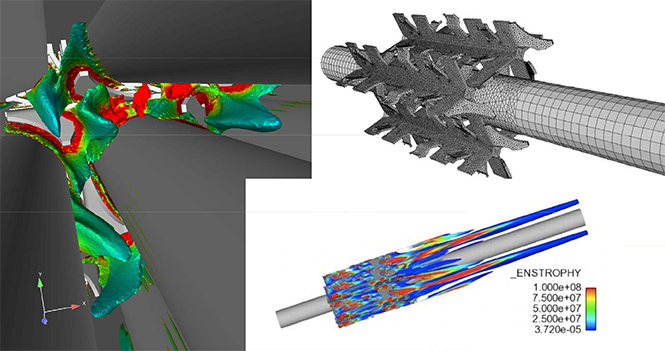
\includegraphics[width=2.5in]{drekar1.png}
        \end{center}
      \end{figure}
    \end{column}

    \begin{column}{0.5\textwidth}
      \begin{figure}[htpb!]
        \begin{center}
          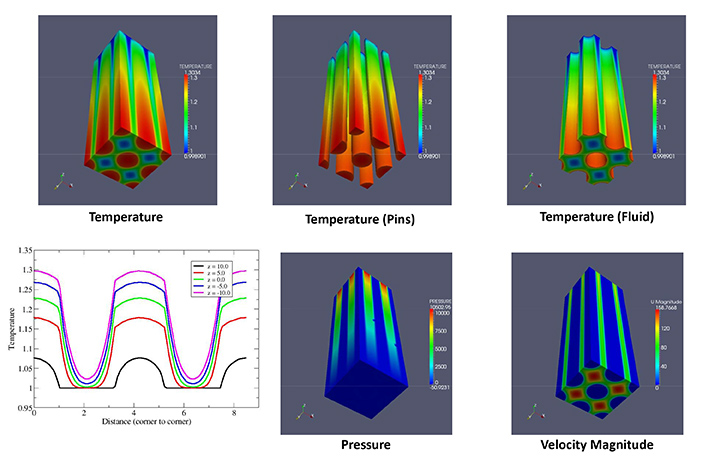
\includegraphics[width=2.5in]{drekar2.png}
        \end{center}
      \end{figure}
    \end{column}
  \end{columns}

  \begin{itemize}
  \item CASL has utilized the Drekar multiphysics code (SNL)
  \item Coupled fluid flow and heat transfer helps characterize many
    phenomena
  \item Drekar is massively parallel and leverages Newton-Krylov
    methods
  \item Propose using the largest Drekar problem to date as a
    challenge problem for the new Monte Carlo methods
  \end{itemize}

  {\small \sl Images source: www.casl.gov}

\end{frame}

%%---------------------------------------------------------------------------%%
\begin{frame}{Conclusion}

  \begin{itemize}
  \item Proposed research and development of new Monte Carlo methods
    \begin{itemize}
    \item Parallelization of Monte Carlo methods for linear systems
    \item FANM for nonlinear systems
    \end{itemize}
  \item Verification through benchmarks
  \item Numerical experiments for understanding
  \item Challenge problem for application
  \item Directed towards hard problems in nuclear reactor analysis:
    \begin{itemize}
    \item Application to multiphysics
    \item Potential improvements for scalability
    \item Potential improvements for memory consumption
    \item Looking forward to exascale
    \end{itemize}
  \end{itemize}

\end{frame}

%%---------------------------------------------------------------------------%%

\end{document}
